%%____________________________________________________________________________||

\section{``Lost lepton'' background estimation}
\label{sec:ttw}

Once all the signal region selection requirements have been imposed,
the contribution from QCD multijet events is expected to be
negligible, as demonstrated in Sec.~\ref{sec:qcd}. In the absence of
multijet events, the background counts in the signal region arise from
SM processes with significant \met in the final state. In events with
low counts of jets and b-quark jets, the largest backgrounds with
genuine \met are from the associated production of W or Z bosons with
jets, followed by either the weak decays \znunu or \wtaunu, where the
$\tau$ decays hadronically and is identified as a jet; or by leptonic
decays that are not rejected by the dedicated electron or muon
vetoes. The veto of events containing isolated tracks is efficient at
further suppressing these backgrounds as well as the single-prong
hadronic decay of the tau lepton. At higher jet and b-quark jet
multiplicities, top quark production followed by semileptonic weak top
quark decay becomes important.  Residual contributions from processes
such as single-top-quark, $\ttbar$V or $\ttbar$H, diboson, and
Drell-Yan production are also expected. These SM processes are
collectively referred to as the non-multijet backgrounds. 

The ``lost lepton'' background consists primarily of processes
yielding at least one W boson, which decays leptonically and the
result lepton is either outside the experimental acceptance or does
not satisfy requirements related to reconstruction ``quality'' or
isolation. Predominantly, the lost lepton background arises from the
\wj and \ttbar processes, which smaller contributions from processes
such as single top, {\ttbar}V, {\ttbar}H, \etc All these processes,
plus any others that yield non-negligible contributions are estimated
using the \mj control region. (The \mmj sample is reserved to estimate
solely the \znunu\ background.)

\subsection{The ``transfer factor'' method}
\label{sec:tf-method-ttw}

The method used to estimate the lost lepton background relies on the
use of a transfer factor (TF) determined from simulated event samples
to transform the observed event yields in the \mj sample, categorised
according to \njet, \scalht, and \nb, $\nobs^{\mj}(\njet, \scalht,
\nb)$, into an estimate of the lost lepton background for the
corresponding (\njet, \scalht, \nb) category of the signal region,
$\npre^{\ttw}(\njet, \scalht, \nb)$. The categorisation of events
according to \njet, \scalht, and \nb in the \mj control region is
identical to that for the signal region, as defined in
Sec.~\ref{sec:selection}.\footnote{One detail here is that predictions
  are made according to the \scalht categorisation used in the control
  regions (up to 11 bins), but the predictions are then aggregated
  over a range in \scalht to map onto a coarser binning scheme that is
  used in the signal region (up to 5 bins). Further details can be
  found in Sec.~\ref{sec:ht-categorisation}.}  Each transfer factor is
simply a ratio of the yields obtained from Monte Carlo (MC) simulation
for the same (\njet, \scalht, \nb) category of the \mj control and
signal regions:
\begin{equation}
  \label{equ:tf-ratio}
  {\rm TF} = \frac{N_{\rm MC}^{\ttw}(\njet, \scalht, \nb)}{N_{\rm MC}^{\mj}(\njet, \scalht, \nb)} 
\end{equation}

In this way, predictions for the lost lepton background can be made,
based on the \mj control region, as follows:
\begin{equation}
  \label{equ:pred-method}
  \npre^{\ttw}(\njet, \scalht, \nb) = 
  \frac{N_{\rm MC}^{\ttw}(\njet, \scalht, \nb)}{N_{\rm MC}^{\mj}(\njet, \scalht, \nb)} 
  \times 
  \nobs^{\mj}(\njet, \scalht, \nb)   
\end{equation}

The selection criteria for the \mj control region
(Sec.~\ref{sec:selection}) closely resemble those for the signal
region, differing mainly through the use of a muon {\it tag} (that is
ignored in the calculation of jet-based kinematic variables such as
\scalht, \mht, \alphat, \etc) and minimal additional kinematic
requirements (\eg a transverse mass window) to obtain a sample
enriched in \wj and \ttbar events. The same selection criteria are
designed to suppress signal contamination so that unbiased data-driven
estimates for the SM backgrounds in the signal region can be
made. Any signal contamination is accounted for in the likelihood
model (Sec.~\ref{sec:likelihood}). 

Figure~\ref{fig:tf_muToTtw} (App.~\ref{app:ttw}) shows the magnitude
of the transfer factors, typically $\ll 1$, The transfer factors
account for differences between the \mj control and signal due to the
acceptance times efficiency for the reconstructed muon and
extrapolations in kinematic quantities. For example, the dependence on
\njet, \scalht, and \nb is largely attributable to the \alphat and
\bdphi requirements for the signal region (that are not used in the
\mj control region).

Many systematic effects are expected to cancel largely in the transfer
factor. However, a systematic uncertainty is assigned to each transfer
factor to account for theoretical uncertainties and effects such as
the mismodelling of kinematics (\eg acceptances) and instrumental
effects (\eg reconstruction efficiencies). These uncertainties are
discussed below. 

\subsection{\texorpdfstring{\mht}{MHT} templates}
\label{sec:mht-intro}

The transfer factors described above provide an estimate of the lost
lepton background as a function of the (\njet, \scalht, \nb) category,
but inclusive with respect to \mht. However, the analysis utilises the
\mht variable to discriminate effectively between SM background and
\eg a potential contribution from SUSY processes. The \HTmiss
information is incorporated into the likelihood model via an \mht
template per (\njet, \scalht, \nb) category, $N_{\rm
  MC}^{\ttw}(\HTmiss;\; \njet, \scalht, \nb)$, which is equivalent to
dicing the numerator of the TF according to \mht, \ie
\begin{equation}
  \label{equ:pred-method-mht}
  \npre^{\ttw}(\njet, \scalht, \nb, \HTmiss) = 
  \frac{N_{\rm MC}^{\ttw}(\HTmiss;\; \njet, \scalht, \nb)}{N_{\rm MC}^{\mj}(\njet, \scalht, \nb)} 
  \times 
  \nobs^{\mj}(\njet, \scalht, \nb)
\end{equation}
In this regard, the TFs described in Sec.~\ref{sec:tf-method-ttw}
provide an estimate of the normalisation for each \mht template. The
\HTmiss templates are taken from simulation and the validity of the
simulation modelling is tested extensively in the control regions, as
described in Sec.~\ref{sec:mht}. 

\subsection{Sideband normalisation for \texorpdfstring{\wj}{W+jets} and \texorpdfstring{\ttbar}{TTbar}} 
\label{sec:sideband-corrections}

In this section, a procedure is described to derive process-dependent
``sideband corrections'' by means of a binned likelihood fit using
data sidebands to the \mj and \mmj control regions. Various different
data sidebands have been considered. However, the one used in this
procedure is the \HTmiss sideband, defined by $100 < \HTmiss <
200\GeV$.

Corrections to the inclusive cross sections of the dominant processes
in the signal and control regions, namely \wj and \ttbar, as well as
\zmmj and \znunuj, are determined.\footnote{Corrections for the latter
  two processes, \zmmj and \znunuj, are discussed in further \ detail
  in Sec.~\ref{sec:sideband-corrections-zinv}.} These corrections are
derived after all relevant corrections are applied to the simulated
samples. Hence, these corrections are expected to be near unity for
each process given that, for example, the simulated samples are
normalised to the integrated luminosity of the data sets using the
most accurate cross section calculations available, typically NNLO or
better. However, there are various potential sources of bias that may
lead to a non-negligible correction. For example, non-unity
corrections may be due to the limited applicability of inclusive cross
section calculations in the high-\scalht, high-\ETmiss corner of phase
space used in this analysis.

It is important to note that this iteration of the analysis is {\em
  not} sensitive to whether these corrections are applied or not, due
to the way the transfer factors are constructed. The \mj sample, rich
in \wj and \ttbar events, is used to predict the lost lepton
background. Both control regions are constructed and binned to cover a
kinematically similar phase space. Hence, the extrapolations are
minimal and so the corrections have little impact on the transfer
factors.

However, the corrections are still determined and propagated to all
steps of the analysis, as they are relevant for some of the
data-driven derivation of systematic uncertainties, such as the
closure tests (Sec.~\ref{sec:closure-tests}) and cross checks of the
\HTmiss modelling (Sec.~\ref{sec:mht}). Without these corrections, the
derived systematic uncertainties could be (unnecessarily)
inflated. Further, the uncertainty in these corrections are not
propagated, as any inaccuracy is -- by construction -- covered by the
aforementioned data-driven procedures to determine systematic
uncertainties.

The \HTmiss sidebands to the control regions are defined with an
identical acceptance to the control regions (except for the \HTmiss
requirement itself) and the sidebands are binned identically in terms
of \njet, \scalht, and \nb. 

A single floating parameter per dominant process, namely \wj, \ttbar,
and \zllj, encodes the correction for that process (fully correlated
across all bins).  The \wj and \ttbar processes are constrained by the
\mj sideband.\footnote{The \zllj process is constrained by the \mmj
  sideband. The correction derived for \zllj is also applied to the
  \znunu + jets simulated event sample. Details can be found in
  Sec.\ref{sec:sideband-corrections-zinv}.}  The corrections and
uncertainties for \wj and \ttbar, as determined by the fit, are shown
in Table~\ref{tab:sbCorrsFromFit}.

\begin{table}[!h]
%  \scriptsize
  \centering
  \topcaption{Corrections to the inclusive cross sections 
    for SM processes determined from a binned likelihood fit to data
    in the $100 < \HTmiss < 200\GeV$ sideband to the control regions.}  
  \label{tab:sbCorrsFromFit}
  \begin{tabular}
    {clc}
    \hline
    \textbf{Process} & \textbf{Sample} & \textbf{Corrrection} \\
    \hline
%    \wj              & \mj             & $1.21 \pm 0.01$      \\ % no NLO/NISR 
%    \ttbar           & \mj, \mmj       & $0.92 \pm 0.01$      \\ % no NLO/NISR
    \wj              & \mj             & $1.06 \pm 0.01$      \\
    \ttbar           & \mj, \mmj       & $0.93 \pm 0.01$      \\
    \hline
  \end{tabular}
\end{table}

\subsection{Overview of systematic uncertainties}
\label{sec:systematics}

The following sections address the estimation of systematic
uncertainties related to the lost lepton background estimation. All
relevant uncertainties are listed in Table~\ref{tab:systs-ttw}, along with
their representative magnitudes and assumptions on inter-bin
correlations. How the uncertainties are incorporated into the
likelihood model is described in Sec.~\ref{sec:likelihood}. 

\begin{table}[h!]
  \caption{Sources of systematic uncertainty in the transfer factors
    used to estimate the lost lepton background using the \mj control
    region. Also shown are the nuisance parameters and correlation
    scheme, as well as representative magnitudes for the uncertainties
    [\%]. The ``type'' refers to whether the nuisance parameters are
    unique to the lost lepton background or shared with the \znunuj
    background estimate (see Table~\ref{tab:systs-zinv}). 
  }   
  \label{tab:systs-ttw}
  \centering
  \fontsize{8}{9.6}\selectfont
  \newcommand{\cat}{\njet, \scalht, \nb, \mht}
  \begin{tabular}{ llllc }
    \hline
    Source of uncertainty               & Nuisance parameters / correlation   & Magnitude (\%)                       & Type   & Figure                              \\
    \hline
    Finite-size simulated samples       & 1 per (\cat) category               & 1--100                               & Unique & n/a                                 \\
    Minimum bias cross section (pileup) & 1, correlated across \cat           & 0.6--3.8                             & Shared & \ref{fig:tfSyst_pu_muToTtw}         \\
    $\mu_R$ / $\mu_F$ scales            & 1, correlated across \cat           & 2.3--3.6                             & Shared & \ref{fig:tfSyst_scale_muToTtw}      \\
    Parton density functions            & 1, correlated across \cat           & 1.1--2.7                             & Shared & \ref{fig:tfSyst_pdf_muToTtw}        \\
    \wj cross section                   & 1, correlated across \cat           & 0.2--1.4                             & Unique & \ref{fig:tfSyst_wjetxs_muToTtw}     \\
    \ttbar cross section                & 1, correlated across \cat           & 0.0--1.0                             & Unique & \ref{fig:tfSyst_ttbarxs_muToTtw}    \\
    QCD + EWK NLO corrections           & 1, correlated across \cat           & 0.5--5.4                             & Shared & \ref{fig:tfSyst_nlo_muToTtw}        \\
    $N_\textrm{isr}$ (\ttbar)           & 1, correlated across \cat           & 0.8--1.1                             & Unique & \ref{fig:tfSyst_nisr_muToTtw}       \\
    Signal trigger efficiency           & 1, correlated across \cat           & 0.0--3.1                             & Shared & \ref{fig:tfSyst_trigger_muToTtw}    \\
    Lepton efficiency (selection)       & 1, correlated across \cat           & 0.0--2.1                             & Unique & \ref{fig:tfSyst_muonsf_muToTtw}     \\
    Lepton efficiency (veto)            & 1, correlated across \cat           & X--Y                                 & Unique & \ref{fig:tfSyst_leptonveto_muToTtw} \\
    Jet energy scale                    & 1, correlated across \cat           & 3.4--5.5                             & Shared & \ref{fig:tfSyst_jec_muToTtw}        \\
    b-quark tag efficiency              & 1, correlated across \cat           & 0.4--0.6                             & Shared & \ref{fig:tfSyst_bsf_muToTtw}        \\
    b-quark mistag probability          & 1, correlated across \cat           & 0.1--1.4                             & Shared & \ref{fig:tfSyst_bsfl_muToTtw}       \\
%    \alphat + \bdphi extrapolation     & 1 per \njet, 1 per \scalht          & X--Y (\njet), X--Y (\scalht)         & Unique & \ref{fig:closure_AlphaT_bDPhi_mu}   \\
    \alphat extrapolation               & 1 per \njet, 1 per \scalht category & 3.3--9.4 (\njet), 2.1--5.9 (\scalht) & Unique & \ref{fig:closure_AlphaT_mu}         \\
    \bdphi extrapolation                & 1 per \njet, 1 per \scalht category & 2.7--22. (\njet), 1.6--18. (\scalht) & Unique & \ref{fig:closure_bDPhi_mu}          \\
    W polarisation                      & 1 per \njet, 1 per \scalht category & 0.9--6.6 (\njet), 1.5--6.6 (\scalht) & Unique & \ref{fig:closure_WPol_mu}           \\
    Single isolated track veto          & 1 per \njet, 1 per \scalht category & 0.0--10. (\njet), 0.0--13. (\scalht) & Unique & \ref{fig:closure_SITV_mu}           \\
    \hline
  \end{tabular}
\end{table}

Several sources of uncertainty are evaluated.  The most relevant
effects are discussed below, and generally fall into one of two
categories. The first category concerns known theoretical and
experimental effects that are propagated through to the transfer
factors and \HTmiss templates. These are decribed in
Sec.~\ref{sec:mc-variations}. The second category aim to cover
additional (unknown) sources of bias, which are determined from
dedicated ``closure test'' studies that involve confronting transfer
factors determined in the phase space of this search against data in
the control regions. Analogous studies with data are performed to
probe the accuracy of the \HTmiss modelling. Studies concerning this
second category of uncertainties are summarised in
Secs.~\ref{sec:closure-tests} and \ref{sec:mht}.

%These uncertainties will be often referred to as
%\textit{``normalisation uncertainties''}, as opposed to the
%\textit{``\HTmiss template uncertainties''} described in
%Sec.~\ref{sec:syst-on-shape}. The former affect the total number of
%events in each (\njet,~\nb,~\scalht) bin (integrating over \mht),
%while the latter encode the limited knowledge on how these events
%distribute in the \mht dimension. The two sets of systematic
%uncertainties have a separate treatment.

\subsection{Known theoretical and experimental uncertainties}
\label{sec:mc-variations}

A set of corrections are applied to the simulated samples in order to
account for known theoretical and experimental biases, such as jet
energy response, b-tagging efficiency, \etc These corrections are
described in Sec.~\ref{sec:sim-corrs}. These corrections are provided
with uncertainties to cover assumptions in the procedures used in
their derivation. Further sources of uncertainties are also
considered, such as the use of LO generators. The effect of various
uncertainties on the transfer factors and \HTmiss templates is
discussed below.

These sources of uncertainty are each assumed to originate from a
unique underlying source and so the effect of each source is varied
assuming a fully correlated behaviour across the full phase space of
the signal and control regions.

\subsubsection{Minimum bias cross section / pileup}
\label{sec:tfSyst_pu}

Events in simulation are reweighted in order to match the distribution
of the primary vertex multiplicity observed in data
(Sec.~\ref{sec:pileup-reweighting}).  A systematic uncertainty is
derived by propagating the 5\% uncertainty on the minimum bias cross
section used in the reweighting procedure.  The relative change in the
transfer factors under this variation is small, at the few percent
level, as shown in Fig.~\ref{fig:tfSyst_pu_muToTtw}
(App~\ref{app:ttw}).

\subsubsection{Effect of scale and PDF on lepton acceptance}
\label{sec:tfSyst_pdf}

Theoretical uncertainties from choices in the renormalisation and
factorisation scales, as well as the parton distribution function, can
introduce systematic uncertaintes on lepton acceptance. The scales
$\mu_R$ and $\mu_F$ are varied by 0.5 and 2.0. Theoretical
uncertainties from parton distribution function are varied according
to the recommended prescription from PDF4LHC~\cite{PDF4LHC:2015}. The
magnitude of the variations in the transfer factors are small,
typically at the few percent
level. Figures~\ref{fig:tfSyst_scale_muToTtw} and
\ref{fig:tfSyst_pdf_muToTtw} (App.~\ref{app:ttw}) show the behaviour
in the transfer factors for variations in scale and PDF, respectively.

\subsubsection{\texorpdfstring{\wj}{W+jets} and \texorpdfstring{\ttbar}{TTbar} composition}
\label{sec:tfSyst_ttW_composition}

The relative composition of \wj with respect to \ttbar in the \mj
control region differs relative to that in the signal region, due to
the application of different kinematic requirements (\eg \mt in the
control region, \alphat and \bdphi in the signal region). Hence,
uncertainties in the inclusive cross sections for \wj and \ttbar may
result in variations in the transfer factors as a function of \njet,
\scalht, and \nb, as well as the \HTmiss templates.

A correction to the inclusive cross sections is applied via the
procedure described in Sec.~\ref{sec:sideband-corrections}, which
adjusts the normalisation of the simulated \wj and \ttbar event
samples to match the data counts in a \HTmiss sideband that
(otherwise) covers an identical region of phase space to the \mj
control region.

Following this procedure, the normalisation for the \wj process is
varied by twice the relative uncertainty in the latest CMS measurement
of the inclusive cross section, while preserving the {\it sum} of the
\wj and \ttbar (and other residual) contributions integrated across
the full phase space of the signal region and, separately, the \mj
control region, in order to see the effect on the ``shape'' of the
transfer factors and the \HTmiss templates. Similarly, the same same
procedure is repeated for variations in the \ttbar normalisation. The
resulting variations are summarised in
Figs.~\ref{fig:tfSyst_wjetxs_muToTtw} and
\ref{fig:tfSyst_ttbarxs_muToTtw} (App.~\ref{app:ttw}). 

\subsubsection{Missing higher-order corrections in LO \texorpdfstring{\MADGRAPH}{MadGraph}
  samples}
\label{sec:nlo}

The \wj process are generated at leading order with the \MADGRAPH
code. The effect of missing higher-order QCD and EWK corrections are
studied by considering the effect of LO$\rightarrow$NLO corrections,
determined as a function of W boson \Pt and shown in
Fig.~\ref{fig:tfSyst_nlo_muToTtw} (App.~\ref{app:ttw}), on the
transfer factors and \HTmiss templates. These corrections include 
NLO QCD corrections derived using {\MADGRAPH{}5\_a\MCATNLO},
and NLO electroweak corrections derived from theoretical calculations,
as described in Ref.~\cite{monojet_AN_36fb}.

Simulated \wj events are weighted according to these NLO corrections,
and the magnitude of each correction is propagated as an uncertainty
throughout the analysis. Fig.~\ref{fig:tfSyst_nlo_muToTtw}
(App.~\ref{app:ttw}) show the effect on the transfer factors as a
function of the various discriminating variables. Uncertainties are
typically at the percent level and as large as $\sim 5\%$.

%All events in the control and signal regions are categorised
%identically according to \njet and \scalht. The NLO corrections are
%determined based on matrix element calculations that consider up to 3
%(1) radiated partons for QCD (EWK) processes. Hence the calculations
%are not necessarily correct for the high-\njet phase space covered by
%this analysis. Hence, these NLO corrections are not applied directly,
%but instead are propagated as an uncertainty through the
%analysis. Fig.~\ref{fig:tfSyst_nlo_muToTtw} (App.~\ref{app:ttw}) show
%the effect on the transfer factors as a function of the various
%discriminating variables. Uncertainties are typically at the percent
%level and as large as $\sim 10\%$.

\subsubsection{\texorpdfstring{\njet}{Njet}-dependent (``\texorpdfstring{\nisr}{Nisr}'') corrections for \texorpdfstring{\ttbar}{TTbar}}
\label{sec:nisr}

The recommendations from the SUSY group to reweight \MADGRAPH \ttbar
Monte Carlo events according to the number of ISR jets ($N_J^{ISR}$)
identified in the event is described in
Sec.~\ref{sec:nisr}. 

All events in the control and signal regions are categorised
identically according to \njet, hence the analysis is not sensitive to
the $N_\textrm{isr}$ corrections. Regardless, these corrections are
applied to simulated \ttbar event, and half the correction is
propagated as an uncertainty throughout the
analysis. Fig.~\ref{fig:tfSyst_nisr_muToTtw} (App.~\ref{app:ttw}) show
the effect on the transfer factors as a function of the various
discriminating variables. Uncertainties are in typically at the
percent level. 

\subsubsection{Signal trigger uncertainty}
\label{sec:tfSyst_trigger}

The effect of uncertainties in the signal trigger efficiency for the
signal region are studied (Sec.~\ref{sec:triggers}). A systematic is
taken as the difference in the efficiency measured using muon and
electron reference triggers.  The relative change in the transfer
factors is typically 0--3\%, as presented in
Fig.~\ref{fig:tfSyst_trigger_muToTtw} (App~\ref{app:ttw}).

\subsubsection{Lepton trigger / identification / isolation efficiencies}
\label{sec:leptonSyst}

The number of events $N^{\mj}$ in the \mj control region is given by
\begin{equation}
  \label{eq:lepton_eff_mj}
  N^{\mj} = 
  N^\textrm{gen}_\mu \,
  \mathcal{A}_\mu \,
  \varepsilon^\textrm{trig}_\mu \,
  \varepsilon^\textrm{ID}_\mu \,
  \varepsilon^\textrm{iso}_\mu  
\end{equation}
where: $N^\textrm{gen}_\mu$ is the expected number of simulated events
(weighted to the integrated luminosity) containing a generator-level
prompt muon prior to event selection requirements; and
$\mathcal{A}_\mu$, $\varepsilon^\textrm{trig}_\mu$,
$\mathcal{A}_\mu$, $\varepsilon^\textrm{ID}_\mu$, and
$\varepsilon^\textrm{iso}_\mu$, are the muon acceptance and the
trigger, identification, and isolation efficiencies, respectively,
which are assumed to factorise. 

%The number of events $N^\textrm{SR}$ in the signal region is defined
%by
%\begin{equation}
%  \label{eq:lepton_eff_sr}
%  N^\textrm{SR} 
%  \; = \; 
%  \sum_{\ell = \mu,e} \; N^\textrm{SR}_\ell
%\end{equation}
%where $N^\textrm{SR}_\ell$ is the number of events containing a
%generator-level particle $\ell$ in the signal region, and the
%summation is performed assuming $\ell$ is either a generator-level
%prompt muon or electron.

The number of events $N^\textrm{SR}$ in the signal region is given by
\begin{equation}
  \label{eq:lepton_eff_sr}
  N^\textrm{SR} 
  \; = \; 
  \sum_{\ell = \mu,e} 
  N^\textrm{gen}_\ell 
  \; [ \;
  (1-\mathcal{A}_\ell)
  \; + \;
  \mathcal{A}_\ell \,
  (1-\varepsilon^\textrm{trig}_\ell)
  \; + \;
  \mathcal{A}_\ell \,
  \varepsilon^\textrm{trig}_\ell \,
  (1-\varepsilon^\textrm{ID}_\ell)
  \; + \;
  \mathcal{A}_\ell \,
  \varepsilon^\textrm{trig}_\ell \,
  \varepsilon^\textrm{ID}_\ell \,
  (1-\varepsilon^\textrm{iso}_\ell)
  \; ]
\end{equation}
where: $N^\textrm{gen}_\ell$ is the expected number of simulated
events (weighted to the integrated luminosity) containing the
generator-level particle $\ell$ prior to event selection requirements;
and $\mathcal{A}_\ell$, $\varepsilon^\textrm{ID}_\ell$, and
$\varepsilon^\textrm{iso}_\ell$ are the experimental acceptance and
the trigger, identification, and isolation efficiencies for the lepton
$\ell$, respectively. The summation is performed assuming $\ell$ is
either a generator-level prompt muon or electron. The four terms of
Eq.~\ref{eq:lepton_eff_sr} are assumed to factorise and provide
the number of events (containing either a muon or an electron) that
fail requirements on acceptance, trigger, identification, and
isolation, respectively.

The effect of theory related uncertainties on lepton acceptance,
$\mathcal{A}_\ell$, for the \mj control and signal regions is
described in other sections (\eg Sec.~\ref{sec:tfSyst_pdf} for scale
and PDF uncertainties).

The effect of experimental uncertainties in efficiency measurements
related to trigger, identification, and isolation requirements are
dsecribed below for both the \mj sample (Eq.~\ref{eq:lepton_eff_mj})
and signal region (Eq.~\ref{eq:lepton_eff_sr}).

\subsubsection*{Selection efficiencies (\texorpdfstring{\mj}{mu+jets} control region)}

The various efficiencies in Eq.~\ref{eq:lepton_eff_mj} are emulated as
part of the detector simulation. Further, (typically near-unity)
data/simulation scale factors are determined and applied to the
simulated events to ensure the emulated efficiencies match the
corresponding measurements in data.

The muon trigger efficiency $\varepsilon^\textrm{trigger}_\mu$ is
emulated in the simulation. Data/MC scale factors provided by the muon
POG are applied to account for differences in the determination of the
muon trigger efficiency from data and simulation. The scale factors
are near-unity and their uncertainties are at the percent level. 

The Tight working point for identification and relative isolation
requirements are applied, as described in
Sec.~\ref{sec:muon-id}. Data/simulation scale factors provided by the
muon POG are applied. Again, the scale factors are near-unity and
their uncertainties are at the percent level.

Finally, $\eta$-dependent muon tracking scale factors provided by the
muon POG, to cover inefficiencies due to the ``HIP effect'', have been
applied and their uncertainties taken into consideration. Their effect
is typically at the percent level. 

The uncertainties in the scale factors have been propagated through to
the transfer factors and \mht templates. A flat 2\% uncertainty, shown
in Fig~\ref{fig:tfSyst_muonsf_muToTtw} (App.~\ref{app:ttw}), fully
correlated in \njet, \scalht, \nb, and \mht, is assumed to cover the
aforementioned effects.

\subsubsection*{Veto efficiencies (signal region)}

Uncertainties in the signal trigger efficiencies are covered in
Sec.~\ref{sec:tfSyst_trigger}. In terms of vetoing leptons (both muons
and electrons) within the experimental acceptance of the signal
region, the Loose working point for identification and
``mini-isolation'' requirements are applied, as detailed in
Secs.~\ref{sec:muon-id} and \ref{sec:electron-id}. The data/simulation
scale factors are provided by the SUSY scale factor working
group~\cite{twiki-leptonSF}. Again, the scale factors are near unity
with uncertainties of a few percent, which have been propagated
through to the transfer factors and \mht templates. A flat 5\%
uncertainty, shown in Fig~\ref{fig:tfSyst_leptonveto_muToTtw}
(App.~\ref{app:ttw}), fully correlated in \njet, \scalht, \nb, and
\mht, is assumed to cover the aforementioned effects. This uncertainty
is assumed to be anti-correlated with respect to the corresponding
uncertainty in the \mj control region, described above. 

\subsubsection{Jet energy scale}
\label{sec:tfSyst_jec}

The effect of varying the jet energy scale in the \mj and \mmj control
regions is investigated.  The energies of jets used in the analysis
are corrected as a function of their \pt and $\eta$ via the procedure
recommended by the JetMET POG. These corrections have an associated
uncertainty, which is propagated through the analysis.  As the \scalht
and jet multiplicity binning is mirrored in signal and control
regions, the effect of jet energy scale on the transfer factor is
expected to be small.  However, the jet energy scale can still have an
effect due to jets moving in and out acceptance (above and below
$40\gev$). The relative change in the transfer factors is presented as
a function of \scalht and jet category in
Fig.~\ref{fig:tfSyst_jec_muToTtw} (App.~\ref{app:ttw}). The changes
are typically in the range of $3-6\%$.

\subsubsection{B-tagging efficiency and mistag probability}
\label{sec:tfSyst_btag}

Scale factors provided by the BTV POG are applied to the MC samples to
correct for differences in the b-tagging efficiencies and
misidentifications between simulation and data.  The method employed
is based on simple event reweighting as described in
Ref.~\cite{btagSFMethods}.  Events are reweighted according to the
probability of obtaining a particular jet configuration in data and
simulation, as determined by the b-tagging efficiencies computed in
the MC samples and the scale factors measured in data.  Since no
extrapolation is performed in the background prediction across
different \nb multiplicities, the analysis is expected to be robust
against variations in the b-tagging efficiency.  To test this effect
the change in the transfer factors is measured by varying the scale
factors within their uncertainties. The scale factors associated with
b and c jets are varied together (since their measurements are
correlated), while those associated with light jets are varied
separately.  The relative change in the transfer factors is presented
as a function of \scalht and jet category in
Figs.~\ref{fig:tfSyst_bsf_muToTtw} and \ref{fig:tfSyst_bsfl_muToTtw}
(App.~\ref{app:ttw}).  They are typically in the range of $0-2\%$.

\subsection{Systematics uncertainties in transfer factors from closure tests}
\label{sec:closure-tests}

The second category of uncertainty is determined from sets of closure
tests based on data control samples~\cite{RA1Paper2012}.  Each set of
tests targets a specific (potential) source of bias in the simulation
modelling that may introduce an \njet- or \scalht-dependent source of
systematic bias in the transfer factors~\cite{RA1Paper2012}.

The level of closure with respect to data is inspected:
\begin{itemize}
\item as a function of \njet while integrating over \scalht and \nb; 
\item as a function of \scalht while integrating over \njet and \nb;
\item as a function of \nb, while integrating over \njet and \scalht.
\end{itemize}
Any non-closure is covered by a systematic uncertainty based on
summing in quadrature the level of closure and its statistical
uncertainty. The magnitude of the uncertainties are summarised in
Table~\ref{tab:systs-ttw} in Sec.~\ref{sec:systematics}. In the
likelihood model (Sec.~\ref{sec:likelihood}), one log-normal nuisance
parameter is used per \scalht category (\ie correlated over \njet and
\nb) and per \njet category (\ie correlated over \scalht and \nb) for
all sources of uncertainty listed in this section.

\subsubsection{Extrapolation in \texorpdfstring{\alphat}{AlphaT} and
  \texorpdfstring{\bdphi}{biased dPhi}}
\label{sec:tfSyst_alphaT}

Unlike the signal region, events in the \mj control region are not
required to satisfy any requirement on \alphat or \bdphi. Hence, the
accuracy of the modelling of the the \alphat and \bdphi variables are
estimated using the \mj sample. From these estimates, systematic
uncertainties in the extrapolation from the control to the signal
region, due to the differing \alphat and \bdphi requirements, is
derived.

Dedicated closure tests confront data yields in a subsample of \mj
events, satisfying the \alphat and/or \bdphi requirements, against
predictions that are determined using another subsample of \mj events
that satisfy an inverted requirement on \alphat and/or \bdphi. The
subsamples are connected via transfer factors that account for the
extrapolation in the variables. Both subsamples comprise predominantly
\wj and \ttbar events. The signal region requirements on \alphat and
\bdphi are summarised in Table~\ref{tab:alphat-thresholds} in
Sec.~\ref{sec:had-signal}.

The level of closure for an extrapolation in \alphat (only) with the
\mj sample is shown in Fig.~\ref{fig:closure_AlphaT_mu}
(App.~\ref{app:ttw}) as function of \scalht and \njet. Similarly,
Fig.~\ref{fig:closure_bDPhi_mu} (App.~\ref{app:ttw}) shows the same
information for the extrapolation in \bdphi (only). Finally, the level
of closure observed when both \alphat and \bdphi requirements are
simultaneously imposed is summarised in
Fig.~\ref{fig:closure_AlphaT_bDPhi_mu} (App.~\ref{app:ttw}).

Any non-closure in the extrapolation of both \alphat and \bdphi is
covered by a systematic uncertainty, which is defined as the
quadrature sum of the observed non-closure and its statistical
uncertainty (indicated by the blue histogram in the figures). 

%\fixme{CLOSURE FITS!}

\subsubsection{The effect of W polarisation on lepton acceptance}
\label{sec:tfSyst_Wpol}

A data-driven test is introduced to check the modelling of the W
polarisation in simulation.  In this study, based on events in the \mj
control region, the number of $\mu^{+}$ events are used to predict the
number of $\mu^{-}$ events, using transfer factors constructed from
simulation. 
%The polarisation of the W boson has an impact on the prediction of the
%\znunu background using the \mj control region, as explained in the
%following.  The production mechanism of $W$ from pp collisions means
%high $p_T$ $W$ bosons are predominantly left handed \cite{WPol}.  For
%high $p_T$ bosons, this implies that $W^+$ decays to the left handed
%neutrino along its direction of motion while the lepton is pointing
%backward. The opposite behaviour is expected for the $W^-$. The lepton
%is therefore more boosted (and the neutrino less boosted) in $W^+$
%decays than $W^-$ decays.  This leads to a larger number of $W^+$
%decays in the single lepton control regions (which relies on the
%lepton $p_T$ for acceptance) than in the signal region (which relies
%on the neutrino $p_T$ for acceptance).
The closure tests are shown in Fig.~\ref{fig:closure_WPol_mu} as a
function of \scalht and \njet. The systematic uncertainties are
typically in the range $\lesssim 5\%$.

\subsubsection{The single isolated track veto}
\label{sec:tfSyst_SITV}

A data-driven test is introduced to check the modelling of the single
isolated track veto, which is applied in the signal and all control
regions of the analysis.

The study is performed in the \mj sample. The single isolated tracks
(SITs) are identified ignoring the reconstructed muon. A subsample of
events containing no SITs is used to predict the event count for a
subsample containing at least one SIT. 

The closure tests are shown in Fig.~\ref{fig:closure_SITV_mu} as a
function of \scalht and \njet. A significant bias is observed, in
which the number of events containing SITs are underestimated by $\sim
40\%$, largely independent of \scalht and \njet. 

A study of kinematic distributions related to SITs and event-level
variables has been performed on a subsample of \mj events containing
at least one SIT. Various distributions can be found in
Figs.~\ref{fig:dataMC_SIT_mu} and \ref{fig:dataMC_SITEvent_mu}
(App.~\ref{app:ttw}). No significant discrepancies are observed in
shapes, only normalisation. The data/MC scale factors (1.42) shown in
each plot are consistent with the bias observed in the aforementioned
closure tests.

\subsection{Systematics uncertainties in the \texorpdfstring{\HTmiss}{MHT} templates}
\label{sec:mht}

\subsubsection{Testing the \texorpdfstring{\HTmiss}{MHT} modelling against data}

The lost lepton background estimate per (\njet, \scalht, \nb) event
category, integrated over \mht, is derived from data control regions
according to the transfer factor method, decsribed in
Sec.~\ref{sec:tf-method-ttw} (\eg Eq.~\ref{equ:pred-method}). The
distribution of events as a function of \HTmiss is estimated using
\mht templates determined from simulation, as described in in
Sec.~\ref{sec:mht-intro} (\eg Eq.~\ref{equ:pred-method-mht}).  The
effect of known theoretical and experimental sources of uncertainties
on the background estimates, as a function of \njet, \scalht, \nb,
{\bf and} \HTmiss are studied in
Sec.~\ref{sec:mc-variations}. 

Further, additional (unknown) sources of systematic bias that may
effect the transfer factors are probed with data using the closure
test approach described above. Finally, this section describes an
analoguous data-driven method that is used to identify potential
biases and determine systematic uncertainties in the simulation
modelling of \mht. The method probes the agreement between simulation
and (control region) data. The level of closure as a function of \mht
in each (\njet, \scalht, \nb) bin is used to determine alternative
templates (\ie systematic uncertainties) to cover sources of bias. It
is important to note that these alternative templates systematics are
used in addition to the ``known'' theoretical and experimental
uncertainties described in Sec.~\ref{sec:mc-variations} and provide an
additional level of information with regards to the accuracy of the
simulation modelling. 

The simulated event samples used in this analysis are produced at LO
and so the ability of the simulation to model correctly the dynamical
behaviour of SM processes is limited by the use of tree-level
calculations only.\footnote{This is mitigated, partially, by the
  inclusion of additional radiated partons in the (tree-level) matrix
  element calculation. The number of additional partons is process
  dependent and can be as large as 4 for \eg V + jets production.}
This limitation in the simulated samples may be manifest in the
mismodelling of kinematical variables, such as \HTmiss, especially if
variables are considered over an inclusive phase space, with events
generated over a range of energy scales.

\begin{figure}[h!]
  \centering
  \subfigure[\mj]{
    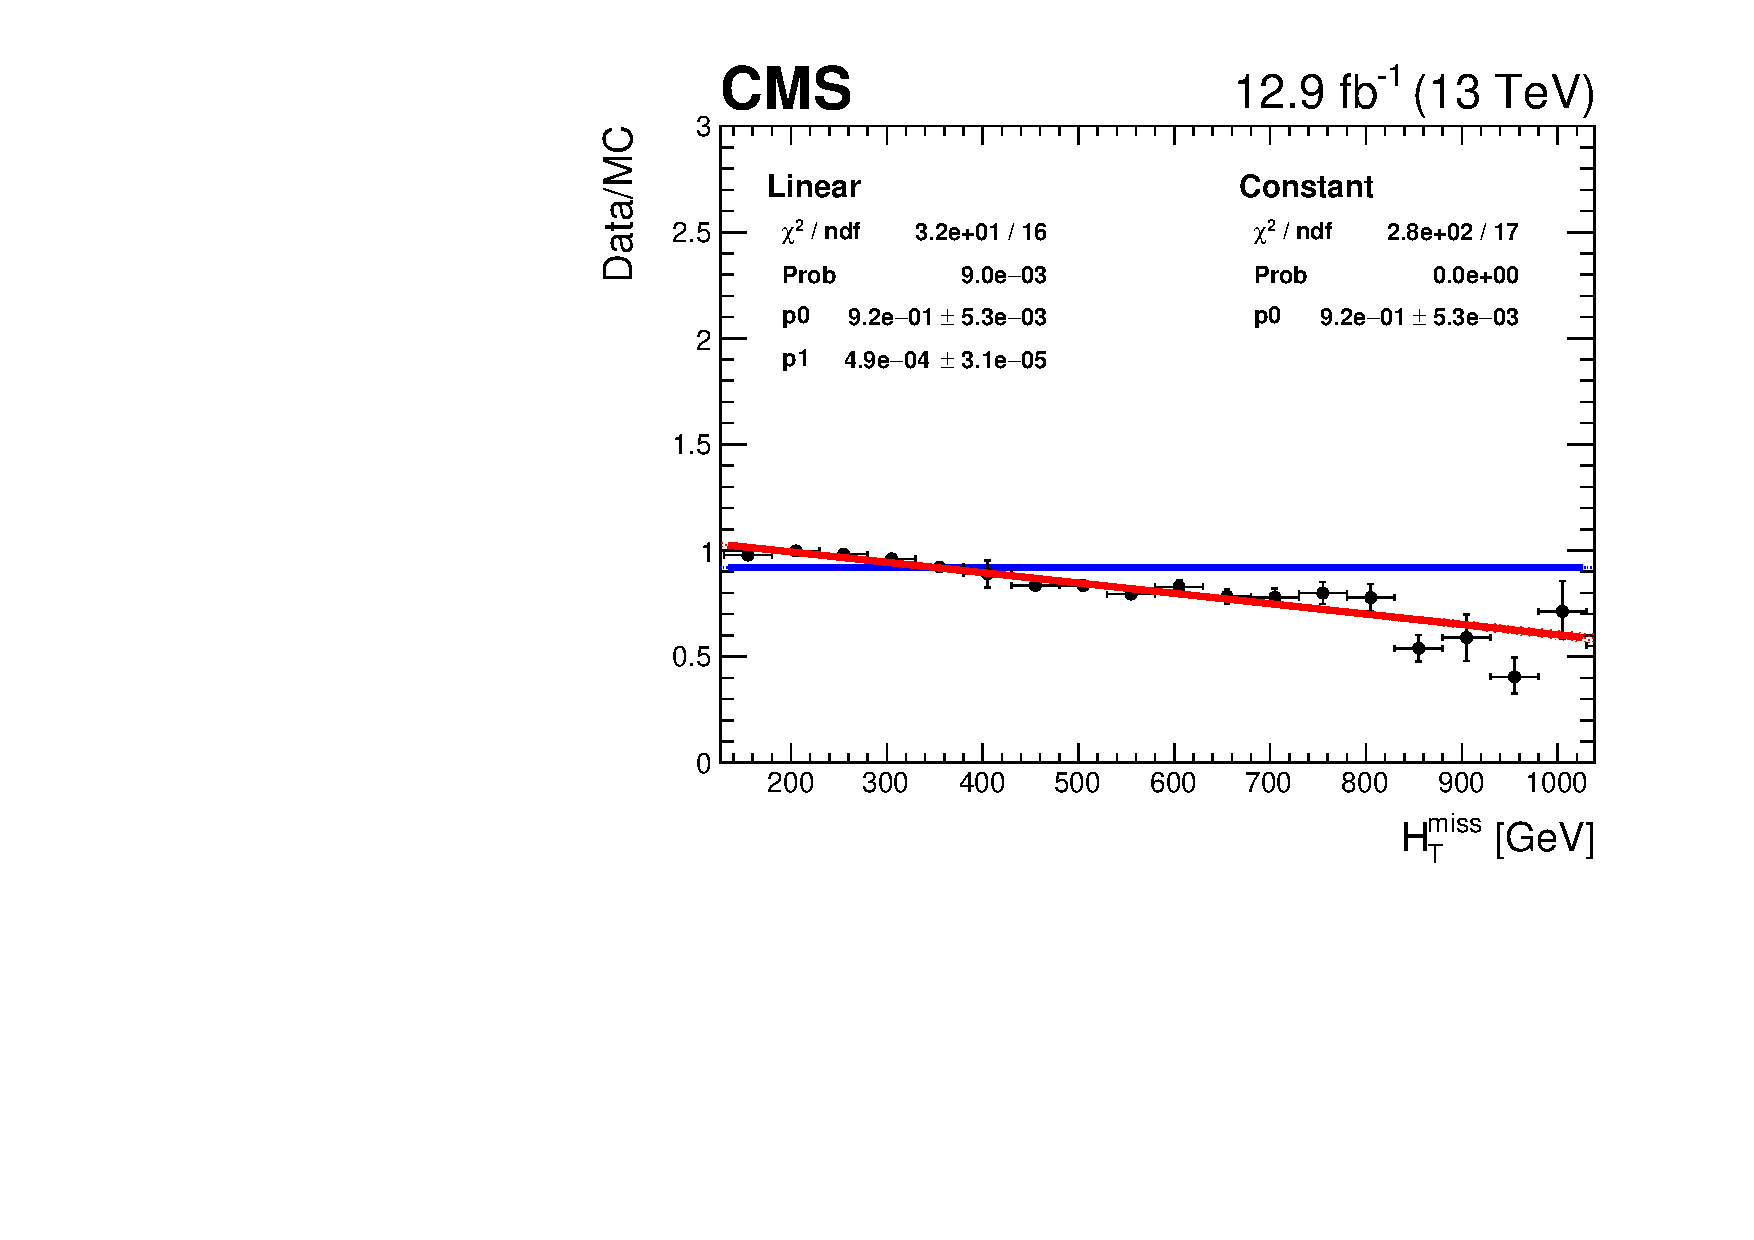
\includegraphics[width=0.5\textwidth]{figures/mhtTemplate/inclusive/mht_Inc_Inc_ht_Inc_SingleMu_Graph.pdf}
  }~
  \subfigure[\mmj]{
    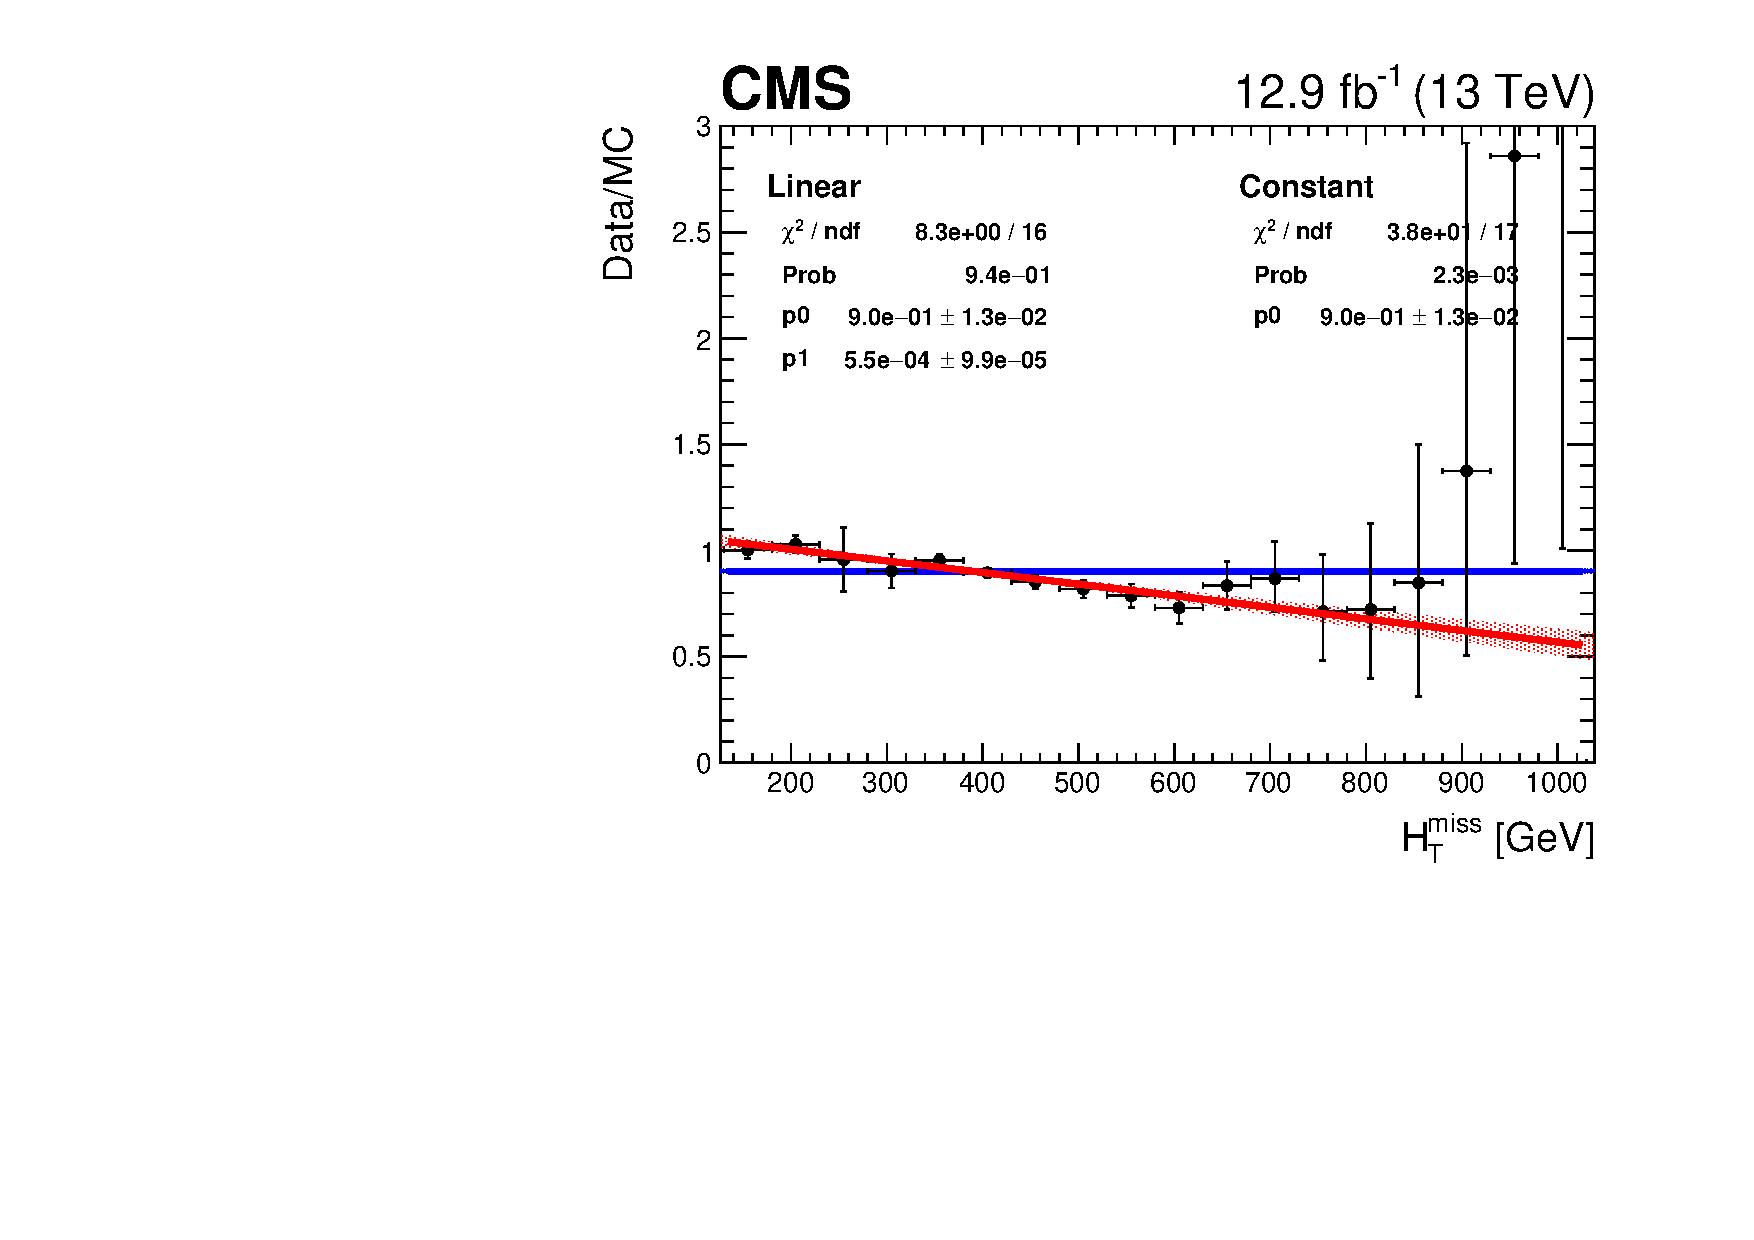
\includegraphics[width=0.5\textwidth]{figures/mhtTemplate/inclusive/mht_Inc_Inc_ht_Inc_DoubleMu_Graph.pdf}
  }\\
  \caption{\label{fig:linearMotiv} The ratio of event yields obtained
    from data and simulation as a function of \mht [GeV] based on a
    sample of (left) \mj and (right) \mmj events that satisfy {\it
      inclusive selection} requirements on \njet and \scalht. Also
    shown are the results of linear fits (\ie first-order orthogonal
    polynomials). No NLO corrections (Sec.~\ref{sec:nlo-intro}) are
    applied to simulated events.}
\end{figure}

Figure~\ref{fig:linearMotiv} shows the ratio of events obtained from
data and simulation as a function of \mht based on a sample of \mj or
\mmj events that satisfy an {\it inclusive selection} on \njet and
\scalht. A significant trend in the ratios versus \HTmiss is observed.

Orthogonal polynomials are used to parameterise the agreement between
data and simulation, such that the odd and even powers of the
polynomial are decorrelated~\cite{cohen2013applied}. The
$n^\textrm{th}$-order orthogonal polynomial is defined in
Eq.~\ref{equ:orthog-polynomial}:
\begin{equation}
  \label{equ:orthog-polynomial}
  f_n(x) = \sum_{k=0}^{k=n}{(p_k)\times(\bar{x}-x)^k}
\end{equation}
where $\bar{x}$ is the weighted mean of the distribution and $p_k = 0$
implies the $k^\textrm{th}$ order term is negligible.

The trend observed in Fig.~\ref{fig:linearMotiv} can be adequately
modelled by a first-order orthogonal polynomial (\ie a linear
function), as indicated by the red line. The fit indicates a
significant trend, which is somewhat expected given that events at
very different energy scales are considered and the ability of the
simulation to model correctly the dynamical behaviour of SM processes
is only known with LO accuracy. The ``flat'' or ``no bias'' hypothesis
(using a zeroeth-order polynomial parameterisation), indicated by the
blue line, is rejected based on a p-value of $\ll 0.05$.

Biases due to limited accuracy in the matrix element calculation for
simulated events may be mitigated if the events are categorised
according to variables that are adequately correlated with the energy
scale of an event, such as \scalht, and the number of additional
partons, such as \njet. In this way, the dynamical behaviour of events
can be {\it measured} with multiple control regions. Once the
simulated events are corrected to data counts in the (\njet, \scalht)
categories (via unconstrained ``rate'' parameters in the likelihood
model, see Sec.~\ref{sec:likelihood}), any potential bias in the
simulation modelling of the \mht variable (as well as any other
\met-like variable) due to energy scale may be mitigated. Other
sources of bias may be the description of the kinematical (rather than
dynamical) behaviour of the SM processes, as well as potential biases
from experimental effects such as jet energy scale and
resolution. This approach is labelled ``scale anchoring'' in the
following discussion. 

The figures in App.~\ref{app:mht} show the ratio of events obtained
from data and simulation as a function of \mht based on a sample of
\mj events that are {\it categorised} according to \njet, \scalht, and
\nb. Note that the \scalht categorisation scheme of the control
regions (Sec.~\ref{sec:ht-categorisation}) is used in this validation
of the \mht modelling. The \nb categorisation is not relevant
for this discussion.

First-order orthogonal polynomials are used to identify significant
trends as a function of \mht via the ``linear'' parameter ($k = 1$),
which is uncorrelated with respect to the ``normalisation'' parameter
($k = 0$). This is done such that the value of the normalisation
parameter can be ignored when attempting to determine biases versus
\mht.\footnote{The normalisation parameter is not relevant for this
  study. Non-unity values are accommodated in the analysis through the
  use of rate parameters in the likelihood model and the transfer
  factor method.}

\begin{figure}[h!]
  \centering
  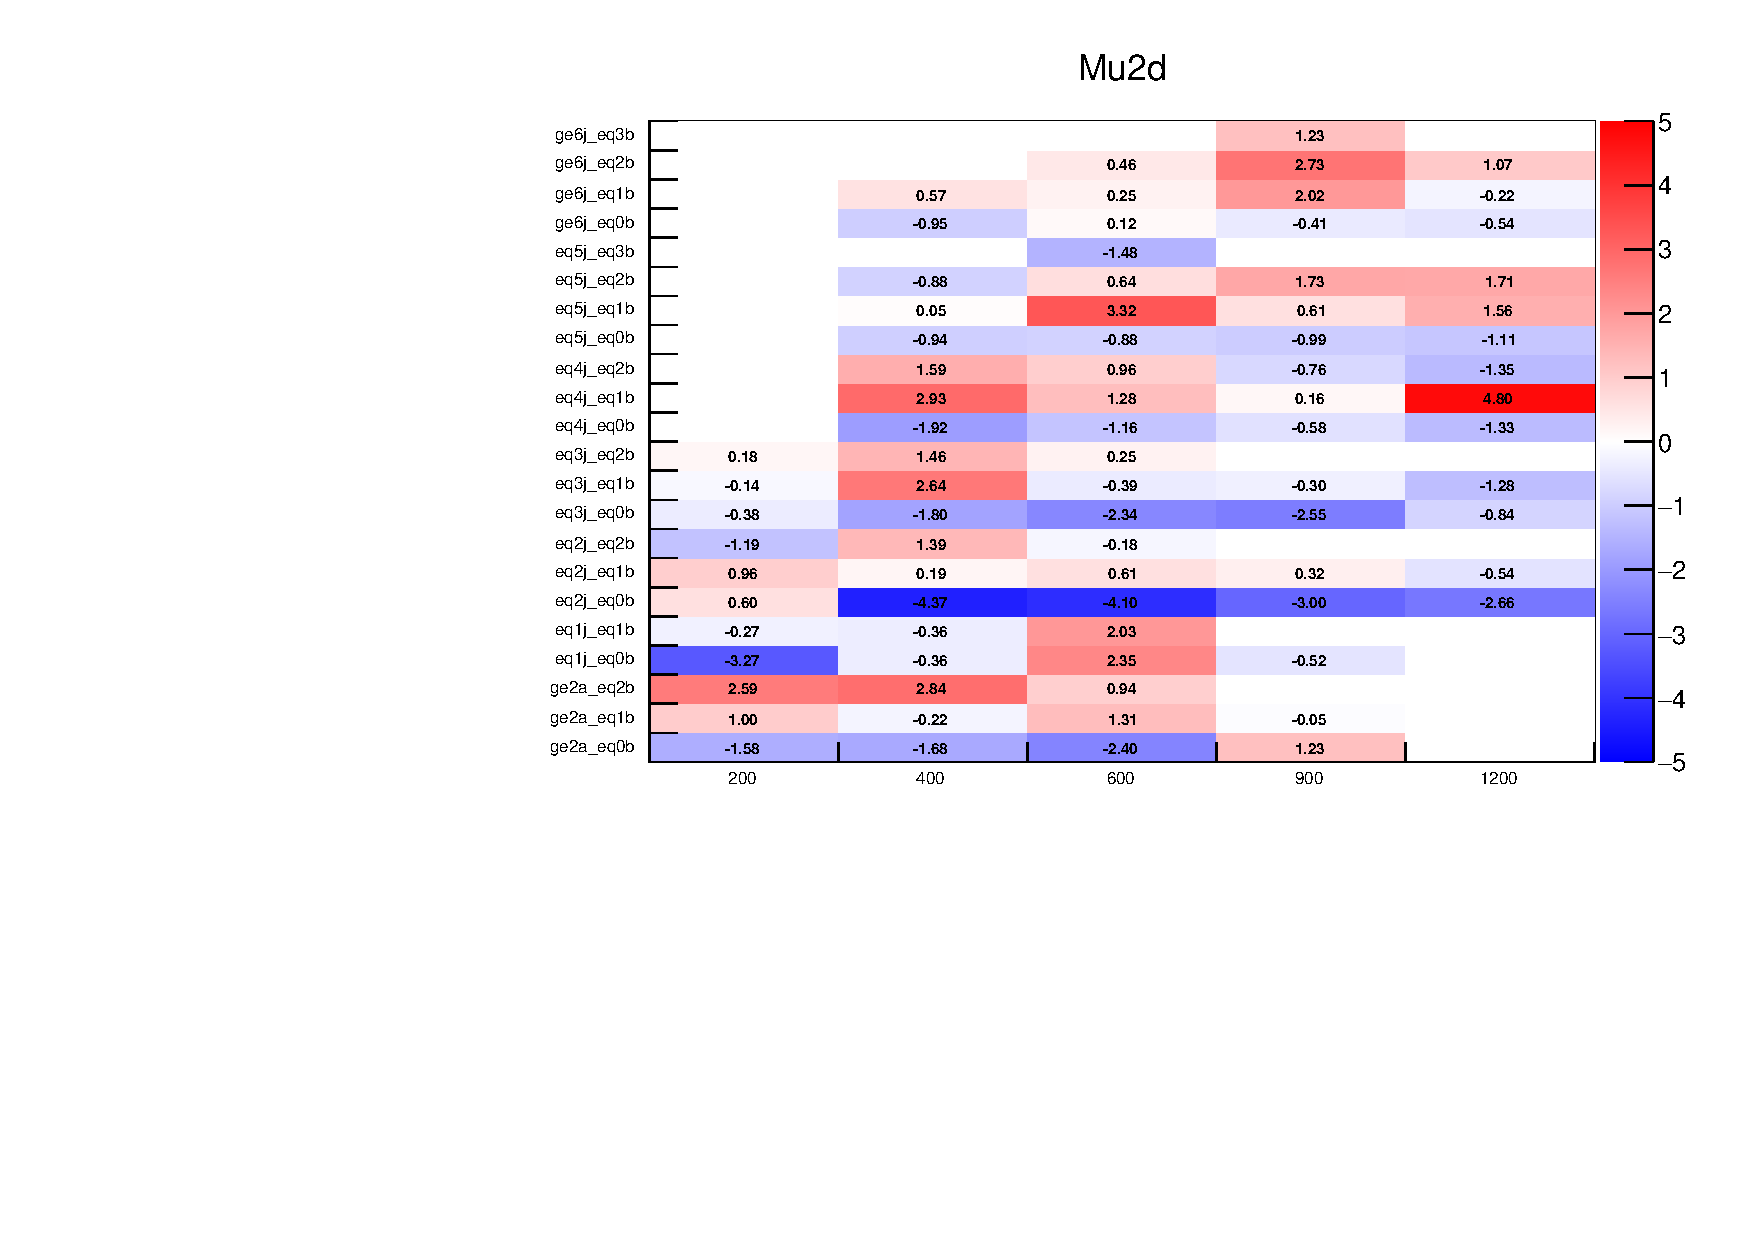
\includegraphics[width=0.5\textwidth]{figures/mhtTemplate/exclusive/Mu_2D}~
  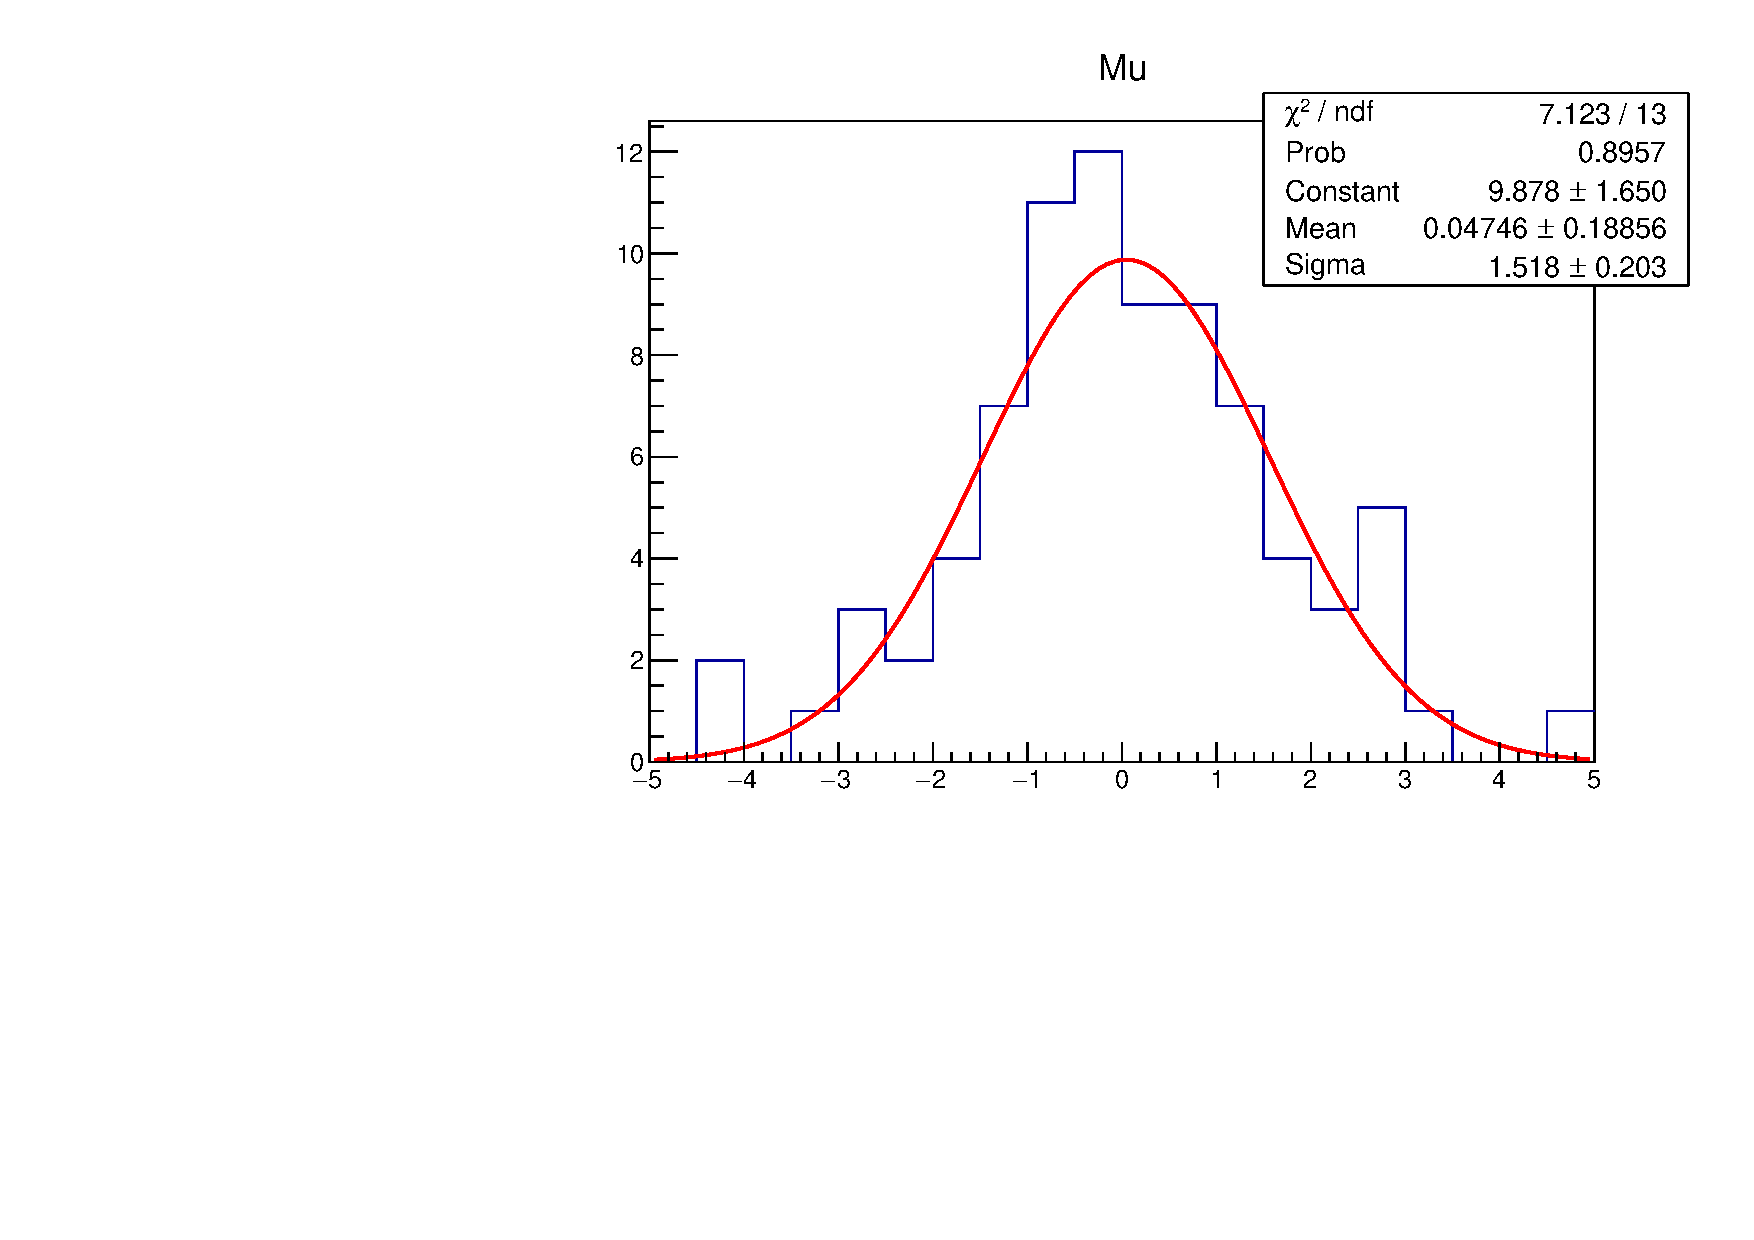
\includegraphics[width=0.5\textwidth]{figures/mhtTemplate/exclusive/Mu}\\
  \caption{(Left) The best fit value for the linear parameter
    relative to unity in units of the associated statistical
    uncertainty, \ie the statistical ``pull'', as a function of \njet,
    \nb, and \scalht. (Right) The histogram of the pull values.}
  \label{fig:pulls} 
\end{figure}

Importantly, in this iteration of the analysis, we now also apply
corrections to simulated event samples as a function of vector boson
\Pt that account for the missing higher-order corrections, namely NLO
QCD and EWK contributions, as discussed in
Sec.~\ref{sec:nlo-intro}. Hence, the ``scale anchoring'' approach now
concerns higher order effects beyond NLO (assuming the NLO corrections
themselves are valid). The following discussion assumes these NLO
corrections are applied to simulated events, unless stated otherwise. 

Following the application of NLO corrections and due to the ``scale
anchoring'' approach, no significant trend as a function of \mht is
expected. The fit information in the figures of App.~\ref{app:mht} is
summarised in Fig.\ref{fig:pulls} (left), which shows the best fit
value for the linear parameter (of the first-order orthogonal
polynomial) relative to unity (\ie no trend) in units of the
associated statistical uncertainty, \ie the statistical ``pull'', as a
function of \njet, \nb, and \scalht. The pulls appear not to exhibit
any structure as a function of \njet, \nb, nor \scalht, and are
approximately gaussian-distributed, with a mean and width compatible
with zero and unity, respectively. This indicates that no large,
significant bias is found in the simulation modelling of the \mht
variable when events are categorised by \njet, \scalht, and \nb. (The
same conclusion is also reached without categorising by \nb.)

This behaviour is consistent with past experience (for which no NLO
corrections were applied). The \HTmiss modelling was inspected in
three data control regions, comprising \mj, \mmj, and \gj event
samples, with the 8\TeV and 13\TeV data sets collected in 2012 and
2015~\cite{Khachatryan:2016dvc}, with no evidence for large,
significant biases.

\subsubsection{Determination of systematic uncertainties}
\label{sec:mht_syst_mu}

Uncertainties in the \mht dimension are extracted using the data
control regions to determine the statistical precision to which the
hypothesis of zero bias can be confirmed. Two sets of systematic
uncertainties in the \mht distributions, correlated in \scalht and
\njet, are determined. The set of systematics decorrelated in \scalht
allows any disagreement to be covered that is localised at a
particular scale, while the set of systematics decorrelated in \njet
covers systematic effects localised in the number of additional
partons. The \nb dimension is not decorrelated as this discriminating
variable is not directly related to the scale of the event and will be
strongly correlated to \njet.

\begin{figure}[h!]
  \centering
  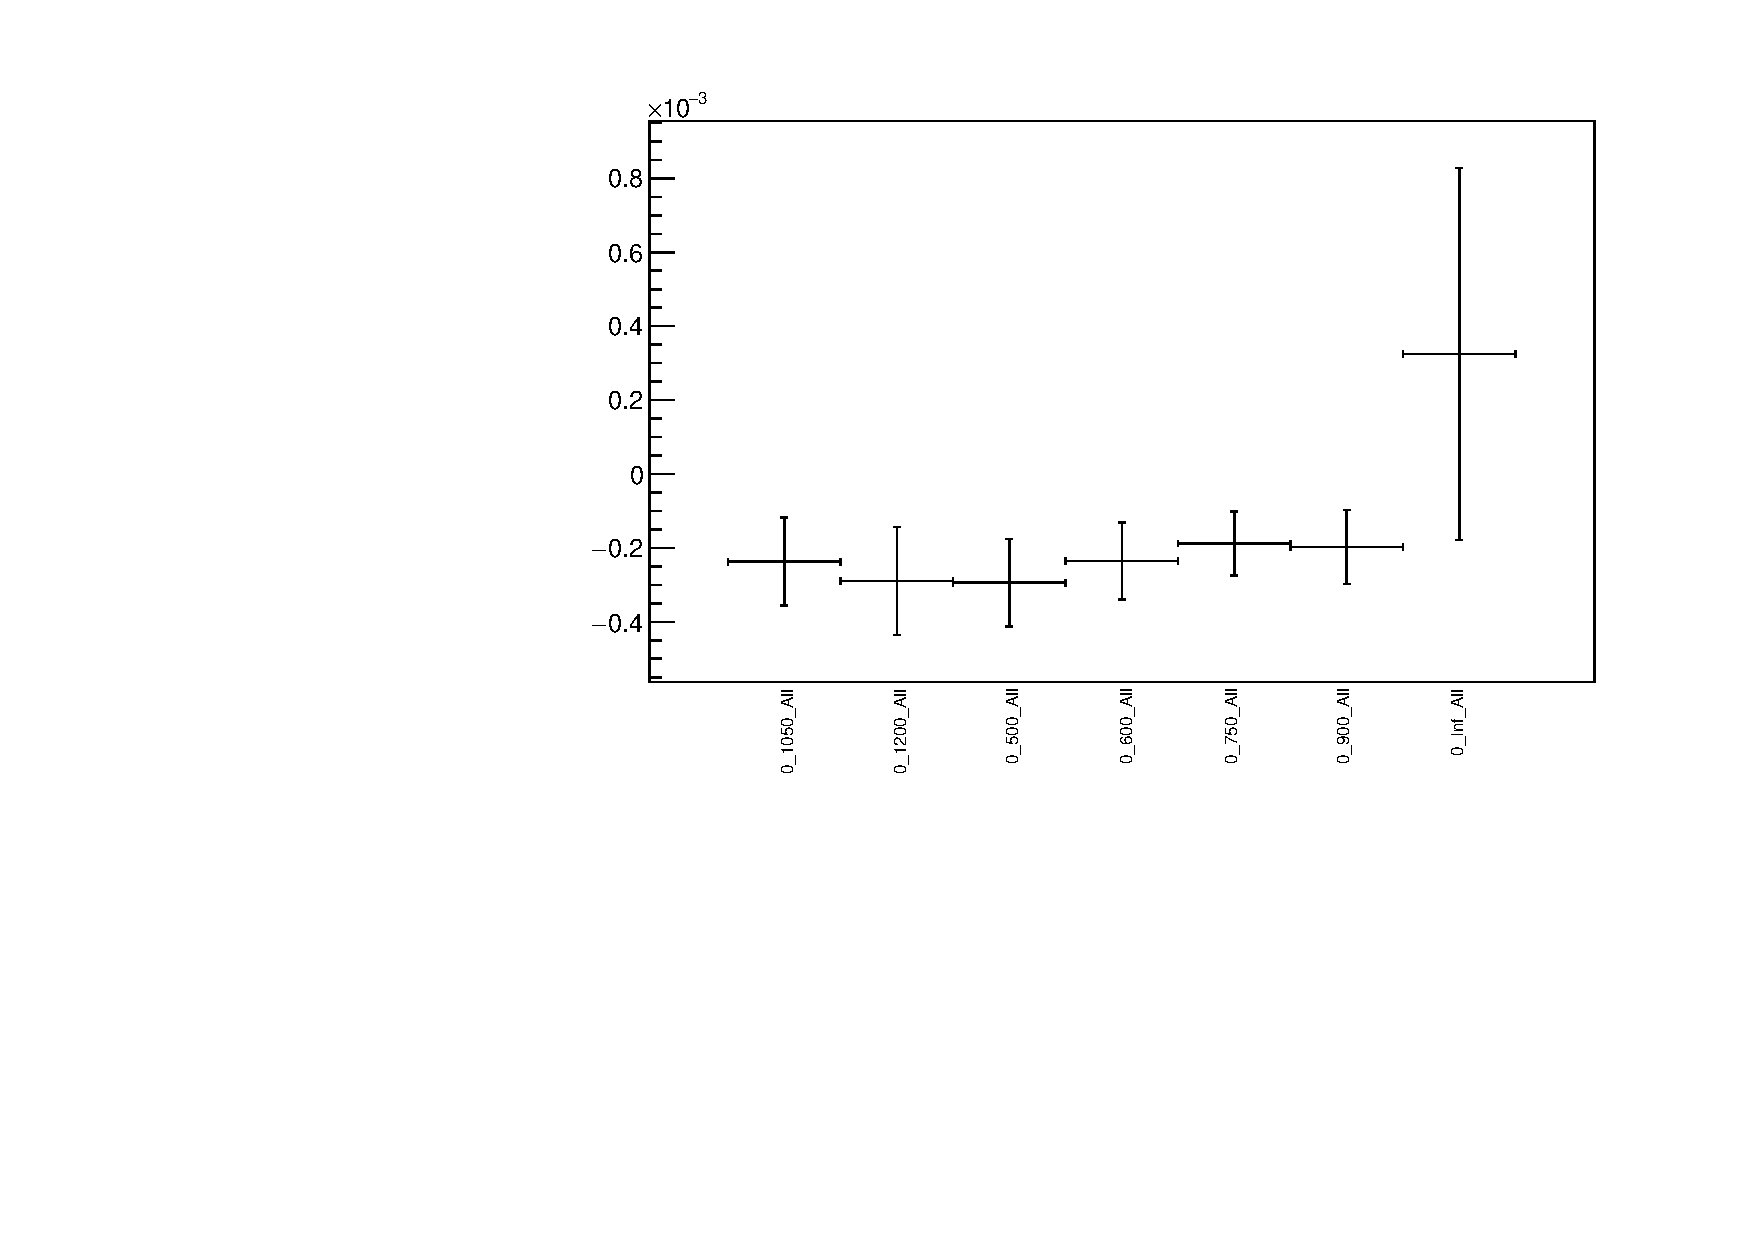
\includegraphics[width=0.5\textwidth]{figures/mhtTemplate/exclusive_corr_njet/Mu_graph}~
  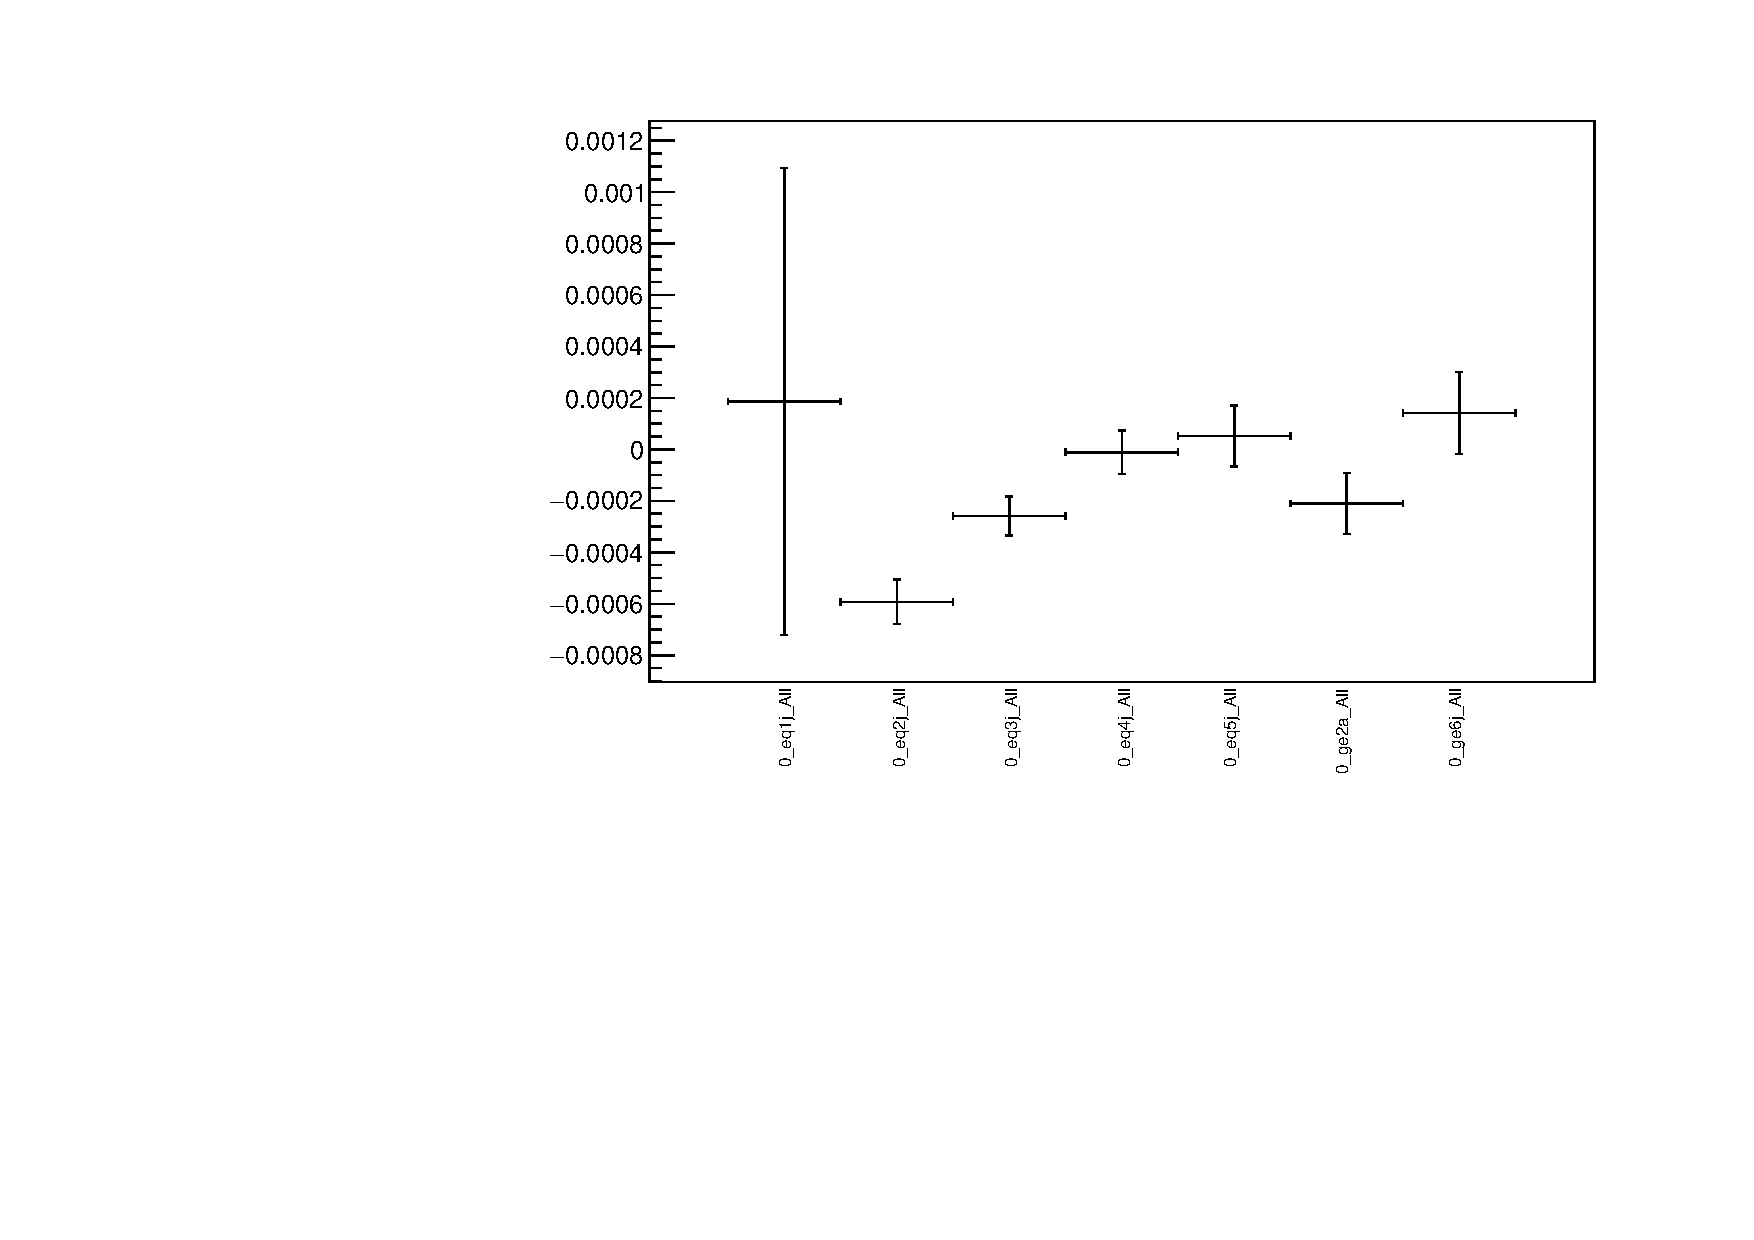
\includegraphics[width=0.5\textwidth]{figures/mhtTemplate/exclusive_corr_ht/Mu_graph}\\
  \caption{\label{fig:postFitMu} Post fit values and uncertainties of
    the linear parameters used to determine the systematics,
    correlated in (left) \njet and (right) \scalht.}
\end{figure}

\begin{figure}[h!]
  \centering
  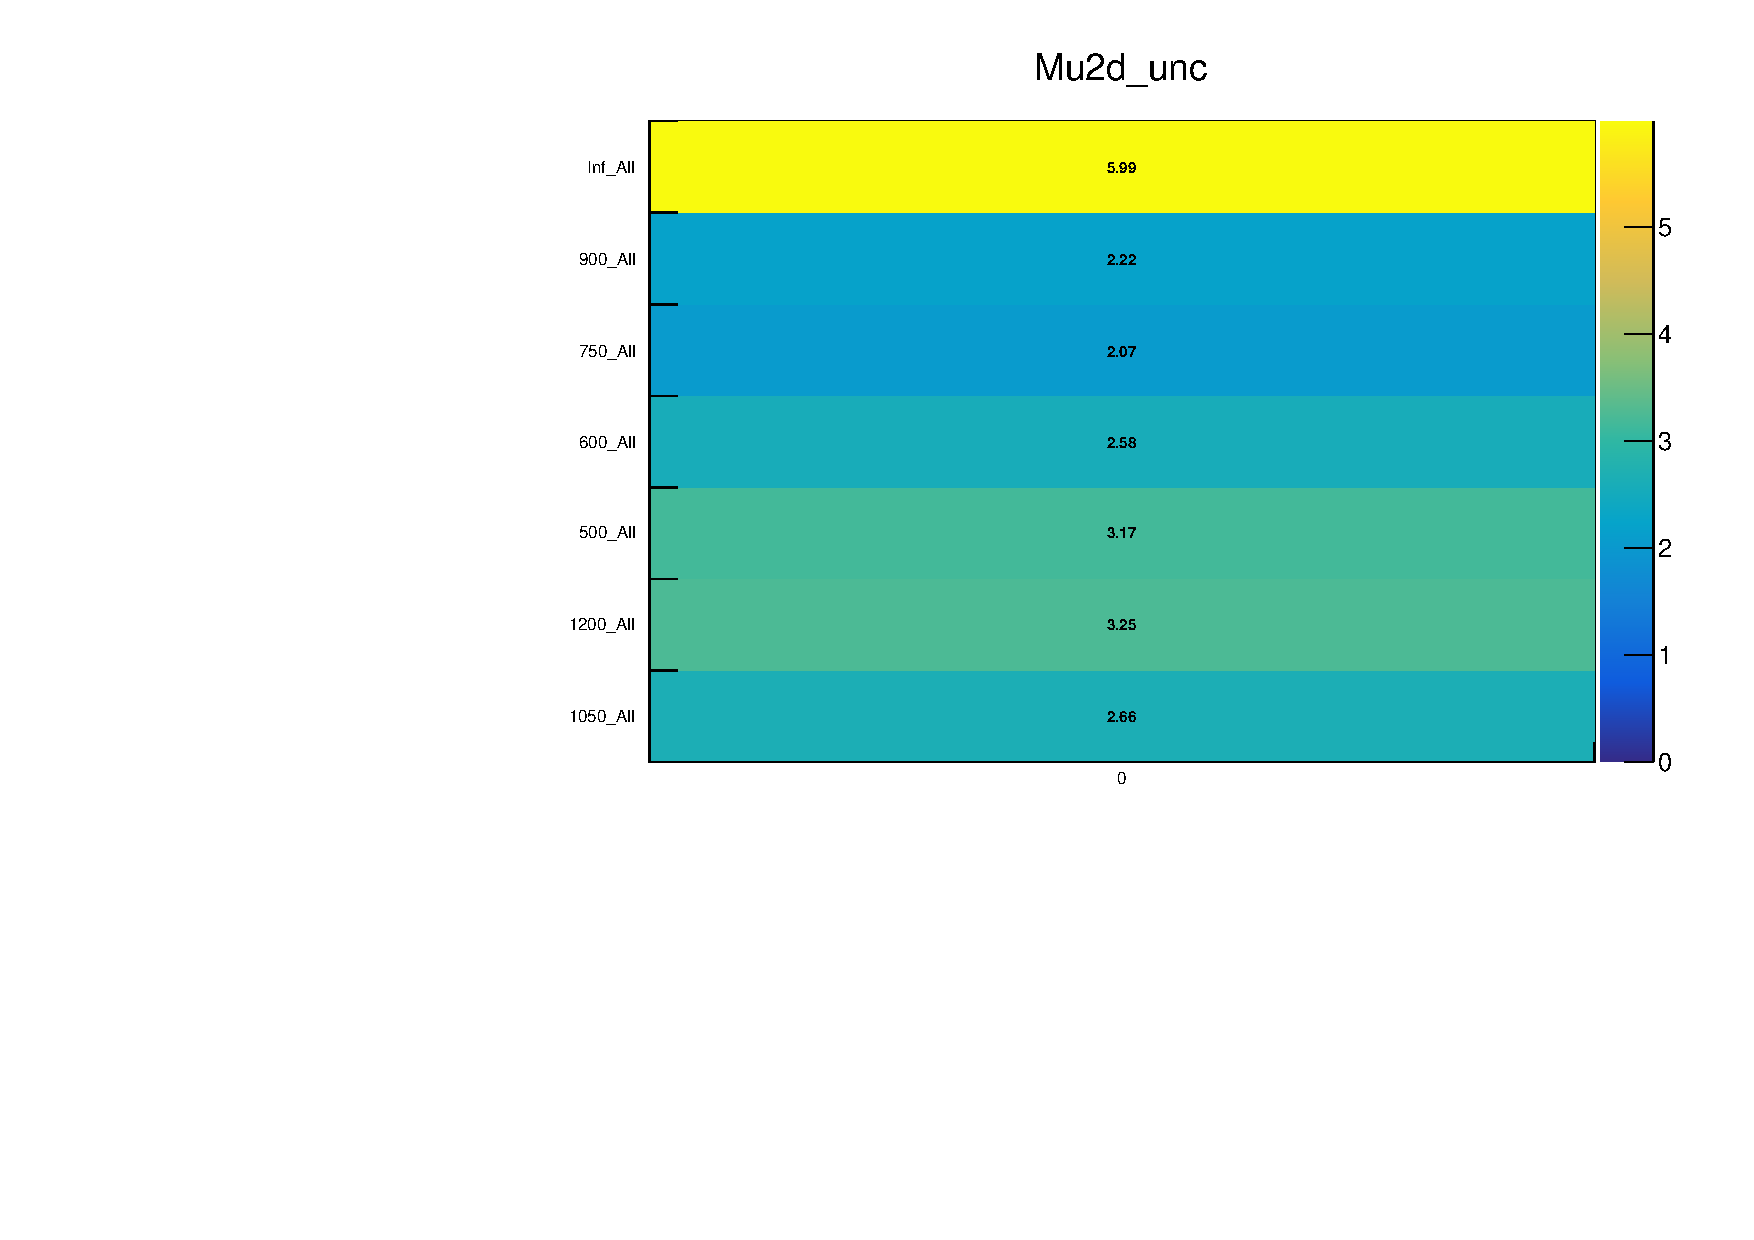
\includegraphics[width=0.5\textwidth]{figures/mhtTemplate/exclusive_corr_njet/Mu_2D_unc}~
  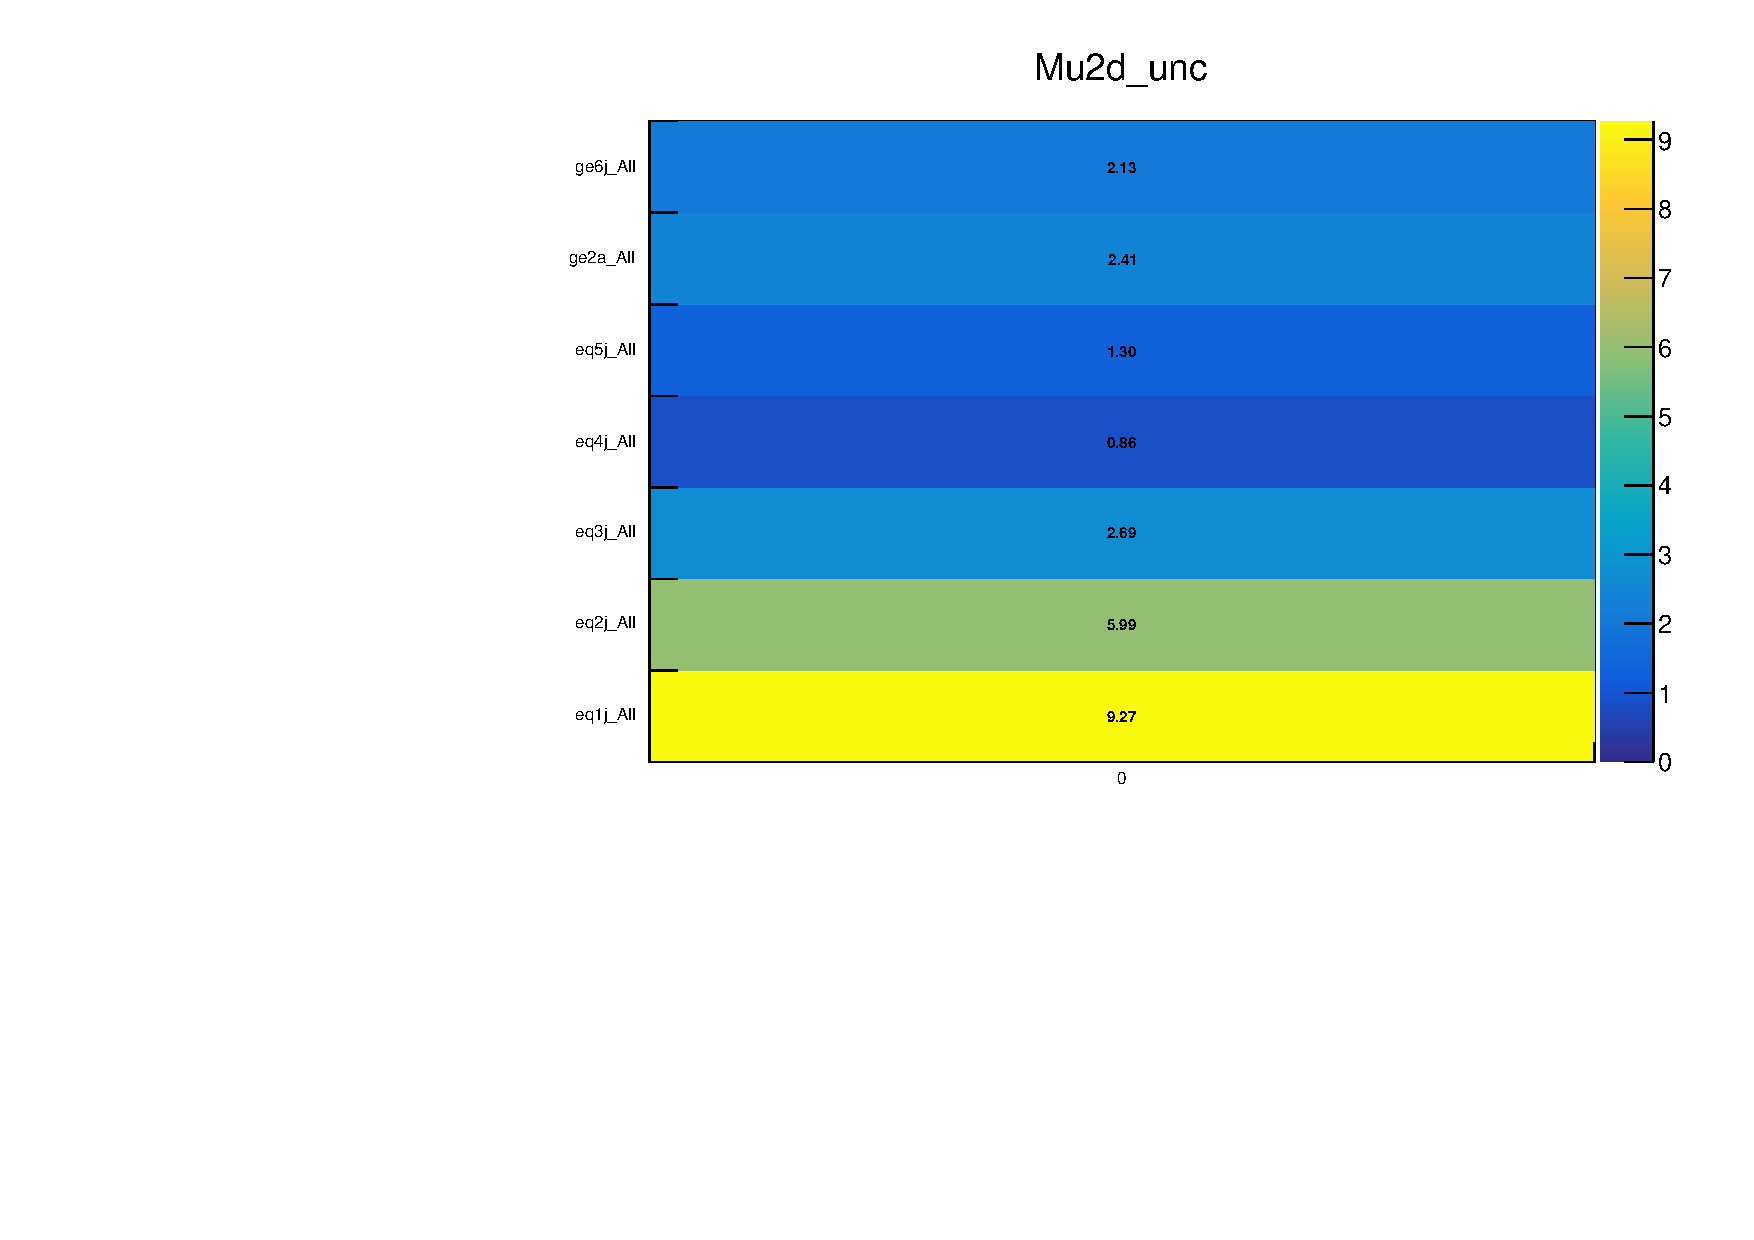
\includegraphics[width=0.5\textwidth]{figures/mhtTemplate/exclusive_corr_ht/Mu_2D_unc}\\
  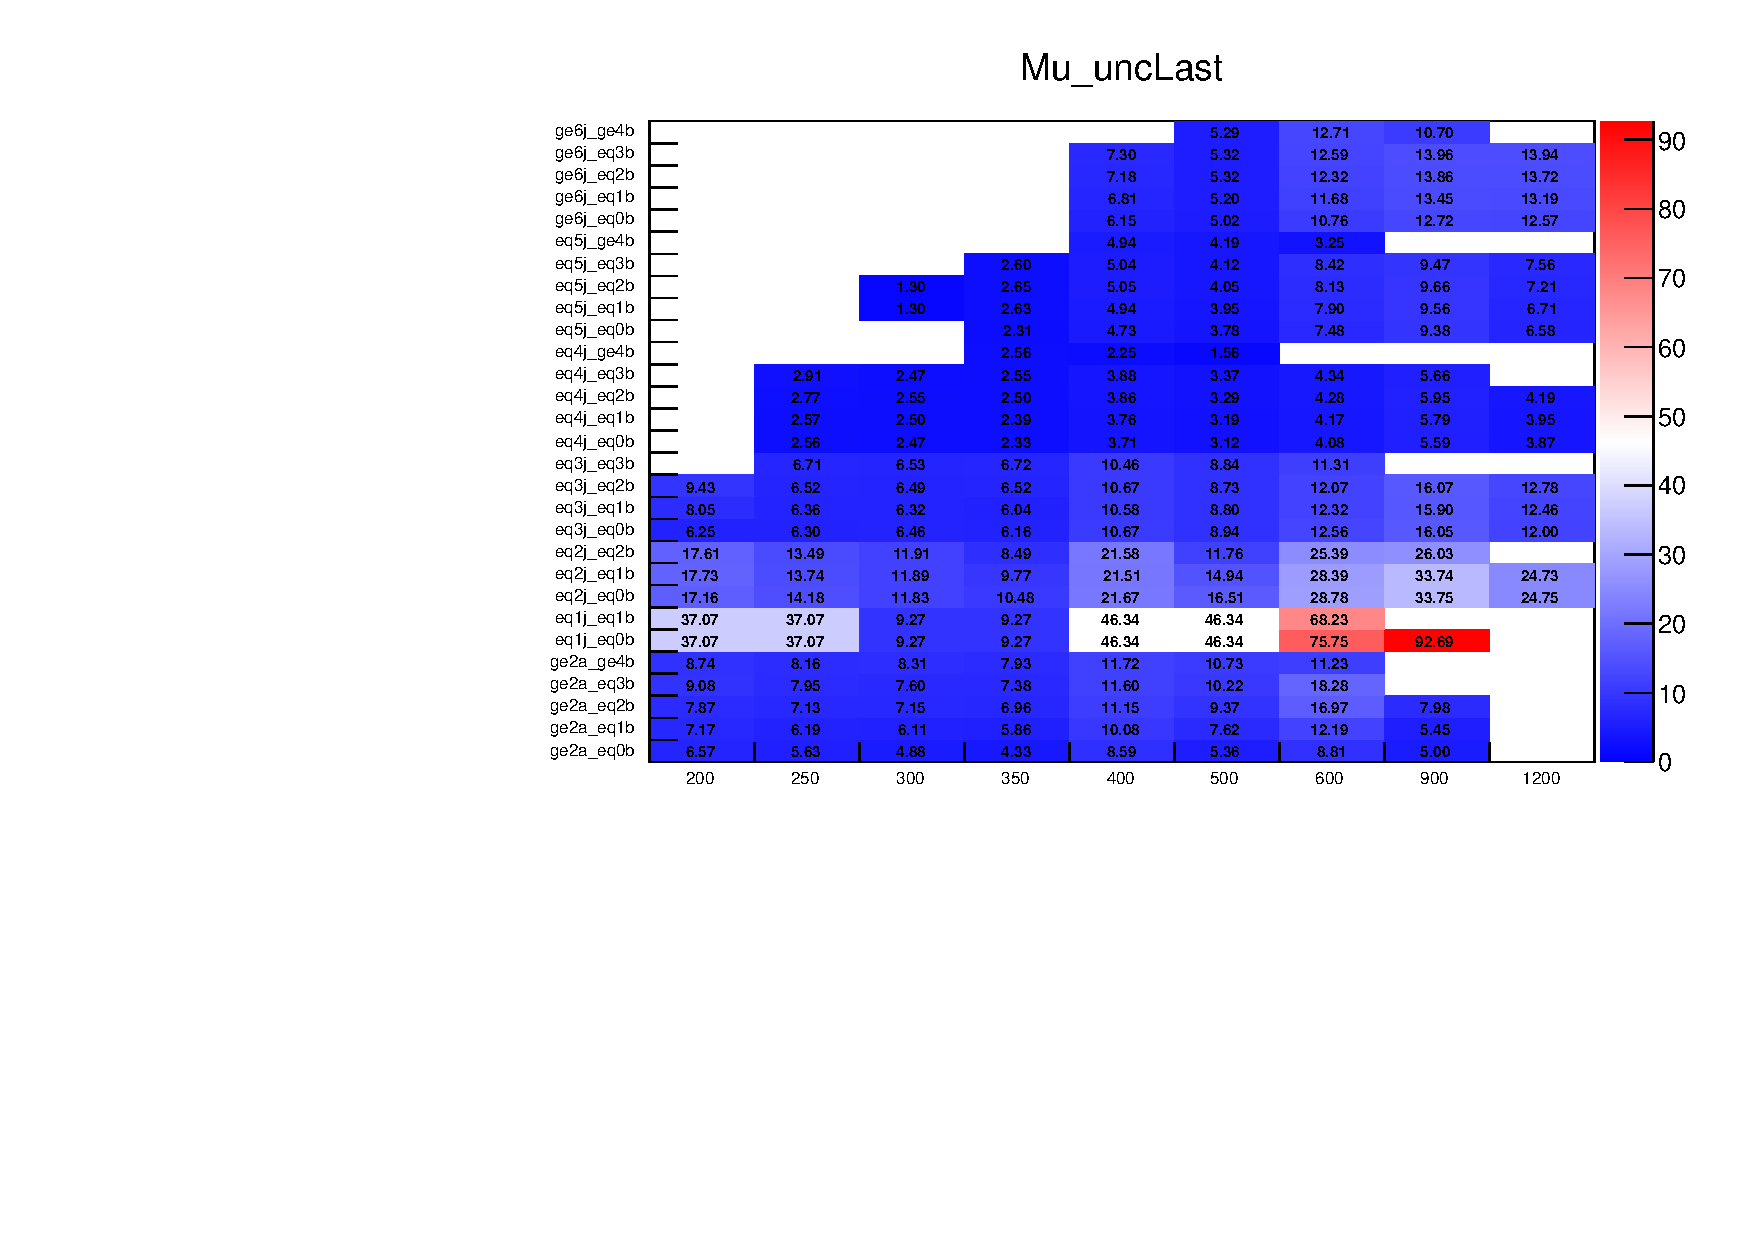
\includegraphics[width=0.5\textwidth]{figures/mhtTemplate/exclusive_corr_ht/Mu_uncLast}\\
  \caption{\label{fig:postFitErrMu} Systematic uncertainties (\%) per
    100\GeV-interval in \mht for effects correlated in (left) \njet
    and (right) \scalht, as determined in the \mj control
    region. (Bottom) Also shown is the systematic uncertainty (\%) in
    the final open \mht bin for each (\njet, \scalht, \nb) category.}
\end{figure}

In order to determine the systematic uncertainties in the \mht
modelling, a linear fit is performed to event yields per (\njet,
\scalht, \nb) event category in the \mj control region. Each fit has
an independent normalisation parameter (\ie uncorrelated across
categories). However, a single linear parameter is used per \scalht
category and shared across \njet categories (\ie correlated across
\njet). A second set of fits are performed with this correlation
pattern reversed: a single linear parameter is used per \njet category
and shared across \scalht categories (\ie correlated across
\scalht). The post-fit values and uncertainties of these linear
parameters are summarised in Fig.~\ref{fig:postFitMu}. The post-fit
value of each parameter is added in quadrature to its uncertainty,
which is used to define $\pm 1\sigma$ variations in the nominal
templates. The alternative templates are added to the likelihood model
with the corresponding correlation pattern.

Figure~\ref{fig:postFitErrMu} shows the systematic uncertainty assumed
per 100\GeV-interval in \mht due to effects correlated in (left)
\njet and (right) \scalht, as determined in the \mj control
region. The values are at the few percent level. Finally,
Figure~\ref{fig:postFitErrMu} also shows the systematic uncertainty in
the final open \mht bin for each (\njet, \scalht, \nb) category, which
is typically at the level of 5--20\%.



